\documentclass[a4paper, draft]{article}
\pagestyle{headings}


\title{Markov chains and Monte Carlo methods - an introduction}

\usepackage{amsmath,amsthm, amsfonts,amscd, amssymb, a4}
\usepackage[final]{graphicx}
\usepackage[final]{listings}
\usepackage{bbm}
\usepackage{empheq}
\usepackage{caption}

\renewcommand\lstlistingname{Algorithm}
\captionsetup[lstlisting]{singlelinecheck=false, margin=0pt, font={sf},labelsep=space,labelfont=bf}



% Numbering

% \numberwithin{section}{chapter}
% \numberwithin{equation}{chapter}

% Theorem environments

%% \theoremstyle{plain} %% This is the default
\newtheoremstyle{own}
    {3pt}                    % Space above
    {3pt}                    % Space below
    {\itshape}                   % Body font
    {}                           % Indent amount
    {\scshape}                   % Theorem head font
    {.}                          % Punctuation after theorem head
    {.5em}                       % Space after theorem head
    {}  % Theorem head spec (can be left empty, meaning ‘normal’)
    
\theoremstyle{own}
\newtheorem{thm}{Theorem}[section]
\newtheorem{cor}[thm]{Corollary}
\newtheorem{lem}[thm]{Lemma}
\newtheorem{prop}[thm]{Proposition}
\newtheorem{ax}{Axiom}[section]

%% \theoremstyle{definition}
\newtheorem{defn}{Definition}[section]

%% \theoremstyle{remark}
\newtheorem{rem}{Remark}[section]
\newtheorem*{notation}{Notation}
\newtheorem{algorithm}{Algorithm}[section]
\theoremstyle{remark}
\newtheorem{example}{Example}[section]

% Fix alignments

% \setlength{\parindent}{0cm}

\newcommand*\widefbox[1]{\fbox{\hspace{4em}#1\hspace{4em}}}
\newcommand*\fullbox[1]{\framebox[\columnwidth]{#1}}

%  Math definitions

% Fields
\newcommand{\R}{\mathbb{R}}
\newcommand{\C}{\mathbb{C}}
\newcommand{\Z}{\mathbb{Z}}
\newcommand{\Q}{\mathbb{Q}}
\newcommand{\N}{\mathbb{N}}
\newcommand{\quat}{\mathbb{H}}

%Groups 
\newcommand{\Lo}{\mathbf{O}(3,1)}
\newcommand{\SL}{\mathbf{SL}}
\newcommand{\SU}{\mathbf{SU}}
\newcommand{\Spin}{\mathbf{Spin}}
\newcommand{\Pin}{\mathbf{Pin}}
\newcommand{\SO}{\mathbf{SO}}
\newcommand{\Poincare}{\mathcal{P}}
\newcommand{\Poincarecov}{\widetilde{\mathcal{P}}}
\newcommand{\Poincareprop}{\widetilde{\mathcal{P}}_+^{\uparrow}}
\newcommand{\Aut}{\mathrm{Aut}}

% Rings
\newcommand{\End}{\mathrm{End}}
\newcommand{\CCl}{\mathbb{C}\mathrm{l}}
\newcommand{\Cl}{\mathrm{Cl}}
\newcommand{\Mat}{\mathrm{Mat}}

% Lie algebras

\newcommand{\spin}{\mathfrak{spin}}
\newcommand{\so}{\mathfrak{so}}
\newcommand{\su}{\mathfrak{su}}
\newcommand{\slc}{\mathfrak{sl}}

%Three-vectors
\newcommand{\xt}{\mathbf{x}}
\newcommand{\yt}{\mathbf{y}}
\newcommand{\pt}{\mathbf{p}}
\newcommand{\nt}{\mathbf{n}}
\newcommand{\sigmat}{\mathbf{\sigma}}

% Vector spaces
\newcommand{\Hil}{\mathcal{H}}

% Other
\newcommand{\calE}{\mathcal{E}}
\newcommand{\calD}{\mathcal{D}}
\newcommand{\calF}{\mathcal{F}}
\newcommand{\calP}{\mathcal{P}}
\newcommand{\Fock}{\mathcal{F}}
\newcommand{\Op}{\mathrm{Op}}

\DeclareMathOperator{\per}{per}
\DeclareMathOperator{\sign}{sgn}
\DeclareMathOperator{\logit}{logit}

\begin{document}
\maketitle

\tableofcontents




\section{A brief introduction to Markov chains}

In this section, we will give a brief introduction into the theory of Markov chains which have far reaching applications to statistics and neuronal networks. We will omit some of the technical details, and refer the reader for some of the available introductions into this topic, for instance \cite{Klenke}, chapter 17 and chapter 18, \cite{RobertCasella1999}, chapter 4, or \cite{MeynTweedie}. We start with the definition of a Markov chain. To prepare the definition, assume that we are given random variables $X_n$. For any $n$, we can then form the conditional probability
$$
P(X_{n+1} \in A | X_1, \dots, X_n)
$$
which is a random variable which is measurable with respect to the $\sigma$-algebra generated by the $X_1, \dots, X_n$. If the random variables take values in some sufficient reasonable space, for instance $\R$, we can apply a factorization and write this random variable as a function of the $X_1, \dots, X_n$. Roughly speaking, a Markov chain is a sequence of random variables for which this conditional probability depends only on the value of $X_n$.  

\begin{defn}\label{defn:markovchain}
Suppose that $\{X_n\}, n \geq 0$ is a sequence of random variables taking values in some measure space $({\mathcal X}, {\mathcal A})$ with a countably generated $sigma$-algebra ${\mathcal A}$. Let us further suppose that $K$ is a {\em Markov kernel} on $\mathcal X$, i.e. a map
$$
K \colon {\mathcal X} \times {\mathcal A} \rightarrow [0,1]
$$
such that for fixed $x \in {\mathcal X}$, $K(x,\cdot)$ is a probability measure and for fixed $A \in {\mathcal A}$, $K(\cdot, A)$ is a measurable function. 
 We say that the $X_n$ form a {\em  Markov chain} if for every $A \in {\mathcal A}$,
 $$
 P(X_{n+1} \in A | X_1, \dots, X_n) = P(X_{n+1} \in A | X_n) = K(X_n,A)
 $$
 i.e. if the conditional probability  $P(X_{n+1} \in A | X_1, \dots, X_n)$ depends only on $X_n$ and $K(\cdot, A)$ is a version of this conditional probability.
\end{defn}

Intuitively, we should think of the index $n$ as describing a time step and the $X_n$ as describing how a random variable $X$ evolves over time. The kernel $K(x,A)$ then describes the probability that the chain will enter $A$ in the next step when $X_n = x$. The elements of ${\mathcal X}$ are often called {\em states}. We will only consider time homogenous Markov chains, where the transition kernel does not explicitly depend on the time $n$, and only Markov chains for which the time index is discrete, however generalisations to continuous times and time dependent kernel exist.

In our definition, we have restricted ourselves to state spaces which are countably generated. This is a usual restriction in the standard literature and is related to the fact that certain results hinge on the availability of a certain class of sets called small sets which is only ensured if the $\sigma$-algebra of measurable sets on the state space is generated by a countable basis, see \cite{MeynTweedie}, Theorem 5.2.1. This assumptions is not overly restrictive, in fact most of our state spaces will either be countable or even finite or will be subsets of some $\R^n$. 

\begin{example}\label{ex:simplerandomwalk}
Suppose that $W_n$ is a sequence of identically distributed and independent real random variables given by a density $w$ called {\em errors}, and that $X_0$ is an arbitrary random variable which is independent from the $W_n$. We can then define a sequence of random variables by
$$
X_{n+1} = X_n + W_n
$$
Then, obviously, the conditional probability $P(X_{n+1} \in A | X_1, \dots, X_n)$ only depends on $X_n$.  We can easily compute these probabilities:
\begin{align*}
P(X_{n+1} \in A | X_n = x_n) = P(W_n \in A - x_n) = \int_A w(x - x_n) d\lambda
\end{align*}
Thus the transition kernel is given by
$$
K(x_n,A) = \int_A w(x - x_n)d\lambda
$$
This type of Markov chain is called a {\em random walk}. It represents a process where each term deviates from the previous term by an error term which is time independent and does not depend on the current state. An example is a game of chance where a player starts with a certain credit 
\end{example}

The following diagram illustrates a random walk with $X_0 = 0$ and $W = {\mathcal N}(0,1)$, the standard normal distribution with mean zero and variance one. We have simulated 3 different runs which are plotted in three different colors, each run consisting of 10000 steps. 

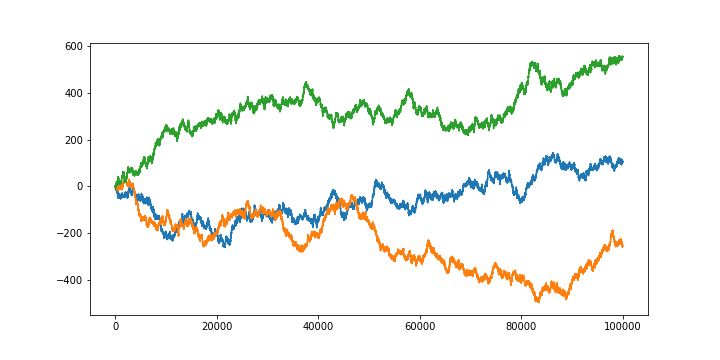
\includegraphics[scale=.47]{RandomWalkSample.png}


As we demonstrate in more detail in section \ref{sec:transitionkernels}, there is a mathematically sound way to define powers of the transition kernel. For instance, we can define a kernel $K^2$ which has the property
$$
K^2(x,A) = \int_{\mathcal X} K(x,dy) K(y,A)
$$
In other words, we take the function on the state space that takes $y$ to $K(y,A)$ and integrate this function over the state space, using the measure $K(x,\cdot)$. As detailed in section \ref{sec:transitionkernels}, this kernel measures the probability that the chain will be in the region $A$ in step two. Similarly, we can define an $n$-th power according to
$$
K^n(x,A) = \int_{\mathcal X} K(x,dy_1) \int_{\mathcal X} K(y_1, dy_2) \dots K(y_{n-1}, A)
$$
Note that this has a very intuitive interpretation. The left hand side is the probability to end up in the set $A$ in step $n$n. To calculate this, we divide the state space into small areas $dy_i$ and sum (i.e. integrate) over all possible paths that start at $x$ and end in $A$, with intermediate steps $y_1, \dots, y_{n-1}$. The mathematically precise formulation of this is via the product and tensor product of transition as described in section \ref{sec:transitionkernels}.

If $\mu$ is a given initial distribution, i.e. if $\mu$ is the distribution of $X_0$, it is not difficult to show (see section \ref{sec:transitionkernels} in the appendix) that this distribution along with the transition kernel fully determines the joint distribution of the $X_i$. We therefore follow the convention to attach the index $\mu$ to an object to indicate that is it refers to the distribution given by $\mu$. If, for instance, $f$ is a random variable depending on the $X_i$ (formally, this would be a random variable on the sequence space ${\mathcal X}^{\Z_+}$), we can take the expectation value with respect to the joint distribution which we will denote by $E_{\mu}(f)$. If $\mu$ is a point measure $\mu = \delta_x$, we also write $E_x$ etc. instead of $E_\mu$. 

\begin{example}
Suppose that we are dealing with a finite Markov chain, i.e. a Markov chain with a finite state space ${\mathcal X} = \{1, \dots, N\}$. Let us also assume that all points are measurable (i.e. we consider ${\mathcal X}$ as a discrete probability space). Then, of course,
$$
K(i,A) = \sum_{j \in A} k(i, \{j\})
$$
Thus we can describe the Markov kernel by a matrix $K_{ij}$ given by
$$
K_{ij} = k(i, \{ j \})
$$
The fact that this kernel is a Markov kernel then implies that for every row index $i$, we have
$$
\sum_j K_{ij} = \sum K(i,\{j\}) = K(i,{\mathcal X}) = 1
$$
Such a matrix is called a {\em stochastic matrix}. What are the products in this case? By the general formula for the product, we have that
$$
K^2(i,\{j\}) = \int K(s,\{j\}) K(i,ds) = \sum_s K(s,\{j\}) K(i,\{s\}) = \sum_s K_{is}K_{sj} = (K^2)_{ij}
$$
In other words, composition of kernels corresponds to matrix products. Thus, the matrix element $K^n_{ij}$ is the probability that after being in state $i$ at a certain step, the process will be in state $j$ after $n$ additional steps. The starting distribution is then given by a row vector $\mu$, defined by
$$
\mu_j = \mu(\{j\})
$$
and the distribution after the first step is then simply $\mu K$:
$$
P(X_1 = j) = \sum_s \mu_s K_{sj}
$$
\end{example}

\begin{example}
Suppose that we are given a finite Markov chain with a state space with only two elements, $1$ and $2$. The Markov kernel is then a 2x2 matrix with row sums one, i.e. is of the form
$$
K = \begin{pmatrix} p & 1-p \\ 1-q & q \end{pmatrix}
$$
Suppose that we start the process in state $1$, i.e. $\mu = (1,0)$. Then after $n$ steps, the process is in state $\mu K^n$. We can now easily simulate this process on a computer. We start with a row vector $\mu$ which is either $(1,0)$ or $(0,1)$. In each step, we compute $\mu K$. We then draw a sample $U$ from a uniform distribution. If $U \leq (\mu K)_1$, we set $\mu = (1,0)$, else we set $\mu = (0,1)$.  The diagram below shows the result of such a simulation, where we have plotted the probability of being in state $(1,0)$ after $n$ steps (i.e. the number of times this state was reached in step $n$ divided by the number of runs), using $p = 0.05$ and $q = 0.2$. Note that $p$ and $q$ are the probabilities in the diagonal, i.e. the probabilities to stay in the state where we are. As these are small, we will - as we can see in the graph - switch between the states in almost all steps. Still the number of times we are in a given state after $n$ steps converges for large values of $n$. The question whether a given Markov chain converges in a certain sense to a target distribution and whether this distribution is unique will be the main focus of this chapter.
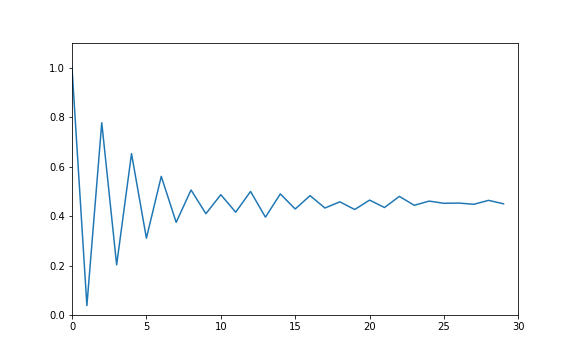
\includegraphics[scale=.55]{TwoDimensionalMarkovChainSample.png}
\end{example}

\begin{example}
Suppose that we are given some random variable $X_0$, a real number $\alpha$ and a sequence of identically distributed and independent random variables $W_n$ called {\em error terms}, which are independent of $X_0$. We can than define a Markov chain by setting
$$
X_{n+1} = \alpha X_n + W_n
$$
As the value of $X_{n+1}$ does only depend on $X_n$ and $W_n$, this is clearly a Markov chain. For the special case $\alpha = 1$, we recover the simple random walk considered in example \ref{ex:simplerandomwalk}. This model is called the {\em scalar autoregression model of order one}. This simple model has an obvious generalisation - we could extend the dependency of $X_{n+1}$ on the other $X_n$ by introducing additional terms, like
$$
X_{n+1} = \alpha_1 X_n + \alpha_2 X_{n-1} + W_n
$$
This is called a scalar autoregression model of order two, and the generalization to higher orders is clear - in a model of order $k$
$$
X_{n+1} = \alpha_1 X_n + \cdots + \alpha_k X_{n-k+1} + W_n
$$
At the first glance, this does not seem to be a Markov chain. However, we can easily build a Markov chain that contains the same information by combining the $X_n$ into a vector with $k$ components. For instance, for $k=2$, we can form the random (column) vector
$$
Y_n = \begin{pmatrix} X_n \\ X_{n-1} \end{pmatrix}
$$
Then 
$$
Y_{n+1} = \begin{pmatrix} X_{n+1} \\ X_n \end{pmatrix} = \begin{pmatrix} \alpha_1 & \alpha_2 \\ 1 & 0 \end{pmatrix}  \begin{pmatrix} X_n \\ X_{n-1} \end{pmatrix}  + \begin{pmatrix} W_n \\ W_{n-1} \end{pmatrix}
= \begin{pmatrix} \alpha_1 & \alpha_2 \\ 1 & 0 \end{pmatrix} Y_n + \begin{pmatrix} W_n \\ W_{n-1} \end{pmatrix}
$$
Thus we see that $Y_{n+1}$ depends only on $Y_n$ and an error term, and hence the $Y_n$ form a Markov chain. This is a very general pattern: a process which remembers $k$ states in the past is equivalent to a Markov chain.
\end{example}

\section{Convergence of Markov chains}

Let us now start to systematically discuss convergence properties of Markov chains. To illustrate this, let us first consider the case of a finite chain described by a transition matrix $K_{ij}$.We have seen that the distribution of $X_n$ is given by $\mu K^n$ where $\mu$ is the initial distribution. So if $K^n$ converges with $n \rightarrow \infty$, we can expect the distribution of $X_n$ to converge as well. If there is a matrix $K^\infty$ such that
$$
\lim_{n \rightarrow \infty} K^n = K^\infty
$$
then of course 
$$
K^\infty K = ( \lim_{n \rightarrow \infty} K^n) K = \lim_{n \rightarrow \infty} K^n K  = \lim_{n \rightarrow \infty} K^{n+1} = K^\infty
$$
In other words, each row $\pi$ of $K^\infty$ will have the property that
\begin{align}\label{def:invariantdistribution}
\pi K = \pi
\end{align}
Interpreting $K$ as transition probabilities, this implies that if the distribution of $X_n$ is $\pi$, the distribution of $P_{X_n}$ will again be $\pi$. Any distribution, described by a row vector $\pi$ with row sum 1, for which equation \ref{def:invariantdistribution} holds is called an {\em invariant distribution}. In other words, invariant distributions correspond to eigenvectors of $K^T$ with eigenvalue 1, and our argument has shown that if $K^n$ converges to $K^\infty$, then every row of $K^\infty$ will be an invariant distribution.

Of course not every kernel leads to a converging Markov chain. If, however, the chain converges and there is an invariant distribution, the question arises whether this is unique. There are obvious examples where this is not the case. Consider the case 
$$
K = \begin{pmatrix} 1 & 0 \\ 0 & 1 \end{pmatrix}
$$
Obviously $K^n = K$ and the chain converges, but every vector with row sum one is an invariant distribution. This chain is too rigid, because in whatever state we start, we will stay in this state forever. It turns out that in order to ensure uniquess of an invariant distribution, we need a certain property that makes sure that the states can move around freely which is called {\em irreducibility}.

Intuitively, we say that a Markov chain is irreducible if any state can be reached from any other state in finitely many steps. For a finite state space, this is rather easy to formalize. A finite Markov chain is called irreducible if, given two states $i$ and $j$, we can find some power $n$ such that
$$
K^n(i, \{ j\}) > 0
$$
Expressing this again in terms of matrices, this amounts to
$$
K^n_{ij} > 0
$$
In other words, given a row index and a column index, we can find a power $n$ such that the element of $K^n$ at $(i,j)$ is not zero. 

Having that notion of irreducibility at hand, we can then search, in a chain which is not irreducible, for sets which are never left once they are entered (called {\em absorbing sets}) and try to split the state space into a collection of these sets and some remaining set. It turns out (see section \ref{sec:irreduciblemarkovchains}) that this can also be done, so that we can restrict most of our attention to irreducible chains.

For general state spaces, our previous definition of irreducibility does not make sense any more, as it relies on the probability to reach a specific point which can be zero in the general case, for instance if we use continuous densities. In this case, there is still a way to define irreducibility. The idea is to introduce an auxiliary measure $\psi$ called an {\em maximal irreducibility measure} and ask that the probability to get from a point $x$ to a set $A$ in a finite number of steps be positive as long as the set $A$ is relevant in the sense that $\psi(A) > 0$. We do not go into the details here but refer the reader to section \ref{sec:irreduciblemarkovchains} in the appendix. If a chain is irreducible in that sense, we call it {\em $\psi$-irreducible}.


Now it turns out that irreducibility alone does itself not yet guarantee a certain stability in the sense of convergence to some stable target distribution. To illustrate the problem, consider the Markov chain given by the transition matrix
$$
K = \begin{pmatrix} 0 & 1 \\ 1 & 0 \end{pmatrix}
$$
Clearly, this chain is irreducible. However, it does not converge - its powers oscillate forth and back between $K$ and $K^2 = 1$. The reason for this is of course the fact that the Markov chain is periodic, i.e. cycles through the same set of states over and over again. So to reach a reasonable convergence, we need to focus on chains that are in a certain sense aperiodic. Again, we have moved the technical details into the appendix (section \ref{sec:periodicmarkovchains}). Basically, the idea is that a chain is aperiodic if it is not forced to cycle through a chain of subsets with probability one. If a chain is not aperiodic, i.e. such a cycle of subsets exists, we can split the state into these subsets and study the subchain that consists of all visits to one of these sets separately. Thus, moving from general chains to aperiodic chains is in some sense again a way to decompose a Markov chain further.
We will now focus on Markov chains that are in that sense fundamental, because neither splitting method applies for them, in other words to irreducible and aperiodic Markov chains.

\begin{example}
Let us consider the following process. We place $N$ points on a circle. We then simulate a Markov chain as follows. We start at some arbitrary point $x$. In each step, we move one point to the left with probability $1/2$ and one point to the right with probability $1/2$. This is obviously a finite Markov chain. If we number the label the points on the circle by $1, 2, \dots, N$, then the transition matrix is given by a matrix of the form (for instance for $N=4$)
$$
K = 
\begin{pmatrix}
0 & \frac{1}{2} & 0 & \frac{1}{2} \\
\frac{1}{2} & 0 & \frac{1}{2} & 0 \\
0 & \frac{1}{2} & 0 & \frac{1}{2} \\
\frac{1}{2} & 0 & \frac{1}{2} & 0
\end{pmatrix}
$$
More generally, we can also allow the process to stay where it is with probability $1 - p$, where $p$ is then the probability to move, which leads us to the matrix
$$
K = 
\begin{pmatrix}
1-p & \frac{p}{2} & 0 & \frac{p}{2} \\
\frac{p}{2} & 1-p & \frac{p}{2} & 0 \\
0 & \frac{p}{2} & 1-p & \frac{p}{2} \\
\frac{p}{2} & 0 & \frac{p}{2} & 1 - p
\end{pmatrix}
$$
We call this process the {\em symmetric random walk on the circle}. Let us study its properties. First, suppose we start at state $1$. We then move to state $2$ with probability $\frac{p}{2}$. From there, we move on the start $3$ with probability 
$\frac{p}{2}$, and therefore the probability that we move from $1$ to $3$ in two steps is at least 
$$
\frac{p^2}{4} > 0 
$$
(in fact, it can be higher, as we can also reach $3$ from $1$ via other paths if for instance $N=4$). Repeating this argument shows that we can get from any point to any other point in a finite number of steps, so the chain is irreducible.
Does it converge to some finite distribution? Let us first inspect the result of a simulation. In figure \ref{fig:CircleRandomWalk}, we have simulated a random walk with $N = 10$ and $p=0.8$, starting at the point $x = 5$. Every picture shows the distribution of the values $X_n$ after running the simulation for an additional 100 steps, so the first histogramm displays the distribution after 100 steps, the second after 200 steps and so forth.

\begin{figure}[ht]
\centering
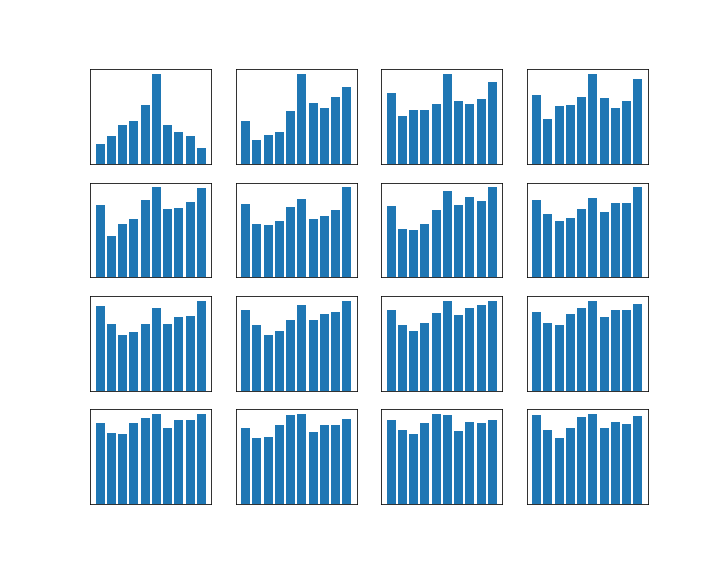
\includegraphics[width=0.7\linewidth]{CircleRandomWalk}
\caption{Random walk on a circle with 10 points and $p = 0.8$}
\label{fig:CircleRandomWalk}
\end{figure}


This does in fact look very much like the chain would converge, and in fact it seems that the chain converges to the uniform distribution. As the matrix $K$ is symmetric, this would imply that the vector
$$
\pi = (\frac{1}{N}, \dots, \frac{1}{N})
$$
is an eigenvector of $K$ with eigenvalue $1$. But this is of course true, as the matrix $K$ has the special property that the values in each of its columns add up to one. 

Let us also visualize how the powers $K^n$ converge. We know that for any state $i$, the $i$-th row of $K^n$ will be the distribution of the $n$-th step of the chain if the chain starts at $i$. In figure \ref{fig:CircleRandomWalkMatrixPowers}, we have displayed all powers $K^n$ for $n = 0, \dots, 15$ in this way. Each colored line corresponds one row of $K^n$. We see that already after a few steps, the plots converge, indicating that the powers of the matrix converge to the matrix with all rows being $\pi$.

Of course we have not proved that the chain really converges, as we have not yet formulated what converge exactly means and how we can derive it. This is the topic to which we now turn.

\begin{figure}[ht]
\centering
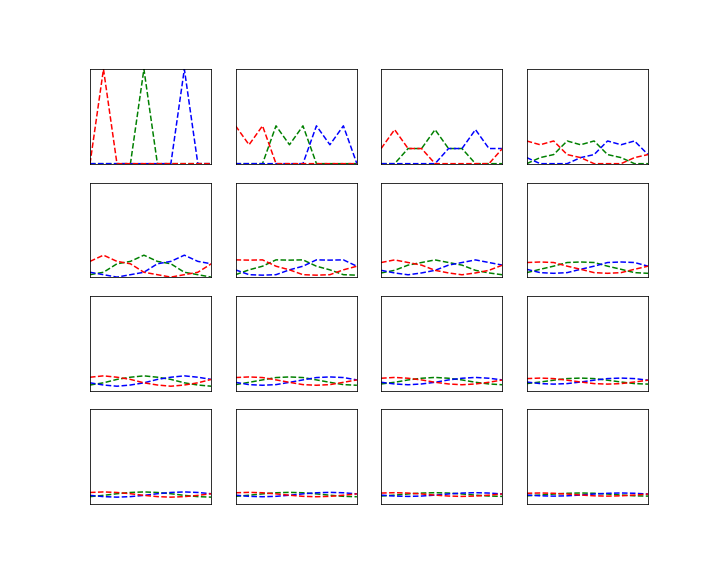
\includegraphics[width=0.7\linewidth]{CircleRandomWalkMatrixPowers}
\caption{Distributions after n steps}
\label{fig:CircleRandomWalkMatrixPowers}
\end{figure}

\end{example}

After having seen an example of converging chain, let us now start to investigate the long-term behaviour of Markov chains in more detail. Given a set $A$, what are the possible ways how the chain can behave with respect to $A$? First, it might happen that the chain returns to $A$ infinitely often and spends an infinite time in $A$. Or, in the other extreme, it might be that the chain eventually leaves $A$ and never returns. In the first case, we say that the set is 
{\em recurrent}, otherwise we call the set {\em transient}. 

It is by far not obvious that these are essentially the only two things that can happen. In the finite case, it is not difficult to show that every irreducible chain is in fact recurrent (see example \ref{ex:finitechainsarerecurrent} in the appendix). For a general state space, it appears to be possible that a chain allows for recurrent as well as transient sets. It is one of the fundamental results of the theory of Markov chains that in an irreducible chain, either all sets are recurrent or all sets are transient (see section \ref{sec:transientandrecurrentmarkovchains}). 


Before we investigate the relation between convergence and recurrence further, let us try to make the idea of stability and convergence of a chain precise. As a motivating example, consider a Markov chain with a finite state space ${\mathcal X}$ and a large, but finite probability space $\Omega$ for which the underlying probability measure is the counting measure. Let $N$ denote the number of elements in $\Omega$. We can think of $\Omega$ as a set of $N$ particles, and of $X_t(\omega)$ as being the state in which particle $\omega$ is at time $t$. Then for each particle $\omega$, the trajectory
$$
t \rightarrow X_t(\omega)
$$
in the state space describes the history of the states through which particle $\omega$ evolves over time. If an initial distribition $\pi$ at time $t = 0$ is given, then
$$
\pi(\{ x \}) = P(X_0 = x) = \frac{ \# \{ X_0(\omega) = x \} } {N}
$$
is the proportion of particles which start their journey at state $x$. At some later time $t$, the proportion of particles in state $x$ is given by
$$
P(X_t = x | X_0 ) = (\pi K^n )(\{ x \})
$$
It is natural to search for an equilibrium, i.e. a distribution such that the number of particles in a given state does not change over time. This does not mean that the state of an individual particle does not change, but is means that the number of particles leaving a state is equal to the number of particles that enter that state at any point in time. The above calculation shows that a distribution is in that sense in an equilibrium state if and only if
$\pi K = \pi$. 
This motivates the following definition. 

\begin{defn}
A $\sigma$-finite measure $\pi$ on the state space of a Markov chain with transition kernel $K$ is called an {\em invariant distribution} or a {\em stationary distribution} if
$$
\pi K = \pi
$$
\end{defn}

Note that we require that the measure $\pi$ be a probability measure or even finite, but we assume that the measure is $\sigma$-finite. 

The question for stability of a Markov chain can then be rephrased in terms of invariant distributions. Thus we would like to know whether an invariant distribution exists, whether it is unique and whether a chain that is in arbitrary intial distribution converges in some sense to the invariant distribution.

One can show (see again the appendix, section \ref{sec:transientandrecurrentmarkovchains}), that recurrence ensures that an invariant measure exists and is unique up to a constant. That measure is not necessarily a finite measure, and can therefore not necessarily be normalized to be probability measure. If it is finite, we call the chain {\em positive recurrent}. Conversely, the existence of an invariant measure implies that the chain is recurrent. Thus we will mainly be interested in recurrent chains.


Let us now define what convergence is supposed to mean. It turns out that a useful mode of convergence is convergence with respect to the total variation norm on the space of measures. 

\begin{defn}
Given a signed measure $\mu$ on a measurable space ${\mathcal X}$, we define the {\em total variation} of $\mu$ to be the number
$$
\| \mu \|_{TV} = \sup \{  \mu(A) - \mu({\mathcal X} - A) \, | \, A \,  \text{measurable}  \}
$$
\end{defn}

We refer the reader to section \ref{sec:totalvariationnorm} in the appendix for some of the properties of the total variation norm.

We now have the terminology in our hands to make convergence of a chain more precise. Given any starting point $x$, we have a sequence $K^n(x, \cdot)$ of probability measures. We can therefore ask whether this sequence converges to an invariant distribution with respect to the total variation norm (which is of course only possible if the invariant distribution is again a probability measure). 


Essentially, this in fact true, at least for almost all starting points $x$. This is the content of the so-called {\em ergodic theorem} for Markov chains which states that under certain regularity conditions (namely irreducibility, aperiodicity and positive recurrence), the chain converges in total variation to the invariant measure $\pi$ for almost all starting points.

To make sure that the convergence happens for all starting points, we need a stronger condition that is called Harris recurrence and which we explore in section \ref{sec:harrisrecurrence} in the appendix, where we have also included a precise statement of the ergodic theorem.




\section{Markov chain Monte Carlo methods}


Having discussed Markov chain from a theoretical point of view, let us now return to an application of Markov chains which is at the heart of many modern numerical approaches to integration and simulation. 

Recall that the term Monte Carlo algorithm typically refers to an algorithm which uses sampling to either simulate outcomes of a random experiment or to approximate integrals. Suppose for instance we are given a finite measure $\pi$ on some state space, say $\R^n$, and we want to compute 
$$
 \int f d\pi
$$
After normalization, we can assume that $\pi$i s a probability measure. Then the integral is the expectation value of the random variable $f$. If we had a method to create an independent and identically distributed series $X_n$ of samples from $\pi$, then the law of large numbers would tell us that for large $n$,
$$
\frac{1}{n} \sum_{k=1}^n f(X_n) \approx \int f d\pi
$$
so that we obtain a good approximation to the integral by generating a sample, calculating the values $f(X_n)$ at the sampled points and taking their average value. This sounds simple, but of course in practice, it can be very difficult to create the required sample.

There are many well known methods to create samples from an arbitrary distribution, like the rejection algorithm or inversion, but most of these approaches do not work well if the dimension of the state space is large. However, there is one class of algorithms that also work well in high-dimensional spaces and that are based on the theory of Markov chains.

The idea behind these methods is rather simple. Suppose we are given a distribution $\pi$ and can somehow construct a Markov chain $X_n$ which converges to $\pi$. Then, assuming that the technical conditions discussed in the last section are fulfilled, we can apply the strong law of large numbers to calculate an approximation to the integral of $f$ from a sample chain $X_n$, even though the $X_n$ are of course neither independent nor identically distributed. We can also use the fact that the distribution of the $X_n$ converges to create a sample from $\pi$. This approach with its ramifications is called the {\em Markov chain Monte Carlo} approach.

Now let us assume that $f$ is an integrable function on the state space. If the random variables $X_n$ where independent and identically distributed, the law of large numbers would tell us that 
$$
\lim_{n \rightarrow \infty} \frac{1}{n} \sum_{k=1}^n f(X_n) \rightarrow E(f)
$$
where the expectation value is taken with respect to the distribution of one - and then each - of the $X_i$. In the case of a Markov chain, the $X_n$ are of course not independent and also not identically distributed. However, if we the distributions $K^n(x,\cdot)$ of the $X_n$ converge to some invariant measure $\pi$, the $X_n$ will, for large $n$, be approximately identically distributed, namely according to $\pi$. Moreover, heuristically we have for large $n, m$ and a fixed starting point $x_0$:
\begin{align*}
P_x(X_{n+m} \in A, X_n \in B) &= \int_B K^m(x,A) K^n(x_0, dx) \\
& \approx \int_B \pi(A) \pi(dx)  
= \pi(A) \pi(B) \\
&\approx P_x(X_{n+m} \in A) P_x(X_n \in B)
\end{align*}
Thus, intuitively, $X_n$ and $X_m$ are almost independent if $n$ and $m$ are large. Thus we might still hope that a relation similar to the law of large numbers still holds, and in fact this is the case. More precisely, if $f$ is some integrable function, we have a convergence
$$
\frac{1}{n} \sum_{k=1}^n f(X_n) \rightarrow \int f d\pi
$$
which again holds for almost all starting points and for all starting points if the chain is Harris recurrent (see section \ref{sec:harrisrecurrence}). These convergence results conclude the theoretical foundations that we need to be able to apply Markov chains in practice.

\section{The Metropolis-Hastings algorithm}

But how do we construct a Markov chain that converges to a given distribution? One approach to this problem is known as the {\em Metropolis Hastings algorithm} and works as follows.

Suppose we are given a finite distribution $\pi$ on a subset ${\mathcal X} \subset\R^n$, which is given by a density with respect to the Lebesgue measure $\lambda^n$ which we again denote by $\pi$, i.e.
$$
\pi(dx) = \pi(x) \lambda^n(dx)
$$
We now choose a {\em proposal density} $q$ on ${\mathcal X}$, i.e. a measurable function 
$$
q \colon {\mathcal X} \times {\mathcal X} \rightarrow [0,\infty)
$$
such that for each $x$, 
$$
\int q(x,y) \lambda^n(dy) = 1
$$
Then $q$ defines a Markov transition kernel 
$$
Q(x,A) = \int_{\mathcal X} q(x,y) \lambda^n(dy)
$$
So far this kernel is not related at all to $\pi$, so we do not consider the Markov chain defined by this kernel. Instead, we now adjust the kernel to reflect the behaviour of $\pi$. For that purpose, define
$$
\alpha(x,y) = 
\begin{cases}
\min \{ 1, \frac{\pi(y)q(y,x)}{\pi(x)q(x,y)} \} & \text{if } \pi(x) q(x,y) > 0 \\
1 & \text{if } \pi(x) q(x,y) = 0 
\end{cases}
$$
The algorithm now works as follows. We start with some arbitrary point $x_0$. When the chain 
has arrived at $x_n$, we first generate a candidate $y$ for the next location from the 
distribution $Q(x_n, \cdot)$. We now calculate $\alpha = \alpha(x_n, y)$. We then accept the proposal with probability $\alpha$, i.e. we draw a random sample $U$ from a uniform distribution
and accept if $U \leq \alpha$. If the proposal is accepted, we set $x_{n+1} = y$, otherwise we set
$x_{n+1} = x_n$.

One aspect that makes this algorithm very appealing is that it only requires to know the densities $\pi$ and $q$ up to a constant, as the constant cancels when we determine the ratios in the above prescription. This is especially appealing in situations where for instance $\pi$ is given in the form
$$
\pi(x) = \frac{\pi^*(x)}{{\mathcal Z}}
$$
where the normalisation ${\mathcal Z}$ is not known, for instance in statistical physics or in a Bayesian setting. Calculating this constant can be very hard, especially in multidimensional settings, and it is very useful that we do not have to determine this constant to apply the Metropolis-Hastings algorithm.

Clearly, the $x_n$ are samples from a Markov chain, as the position at step $x_n$ only depends on the position at step $x_{n-1}$. Before we start to explore the transition kernel of this chain and to investigate under which conditions it converges, let us consider a few special cases to get an idea why this algorithm works. Assume, for instance, that the proposal density $q$ is symmetric, i.e. that 
$$
q(x,y) = q(y, x)
$$
This is the original {\em Metropolis algorithm} as proposed in \cite{Metropolis1953}. If we also assume that $\pi$ and $q$ are nowhere zero,  $\alpha$ simplifies to
$$
\alpha(x,y) = 
\min \{ 1, \frac{\pi(y)}{\pi(x)} \}
$$
Thus we accept the proposal if $\pi(y) \geq \pi(x)$ with probability one. This is very similar to a random search for a global maximum - we start at some point $x$, choose a candidate for a point with higher value of $\pi$ at random and proceed to this point. The major difference is that we also accept candidates with $\pi(y) < \pi(x)$ with a non-zero probability. This allows the algorithm to escape a local maximum much better. Intuitively, the algorithm will still try to spend more time in regions with large values of $\pi$, as we would expect from an attempt to sample from the distribution $\pi$. 

In this form, the algorithm is extremely easy to implement. All we need is a function {\it propose} that creates the next proposal, and a function {\it p} that calculates the value of the probability density $\pi$ at some point. Then an implementation in Python is as follows.

\begin{lstlisting}[frame=single,language=Python,caption=Metropolis algorithm in Python]
chain = []
X = 0
chain.append(X)
for n in range(args.steps):
  Y = propose(X)
  U = np.random.uniform()
  alpha = p(Y) / p(X)
  if (U <= alpha):
    X = Y
  chain.append(X)
\end{lstlisting}

In the diagram below, this algorithm has been applied to a Cauchy distribution with mode zero
and scale one, using a normal distribution with mean $x$ and standard deviation $0.5$ as a proposal for the next location. The chain was calculated for 500.000 steps. The diagram in the upper part shows the values of the chain during the simulation. 

Then the first 100.000 steps were discarded and considered as "burn-in" time for the chain to stabilize. Out of the remaining 400.000 sample points, points where chosen with a distance of 500 time steps to obtain a sample which is approximately independent and identically distributed.
This is called {\em subsampling} and typically not necessary for Monte Carlo integration (see \cite{MCMCHandbook}, chapter 1 for a short discussion of the need of subsampling), but is done here for the sake of illustration. The resulting subsample is plotted as a histogramm in the lower left corner of the diagram. The yellow line is the actual probability density.  

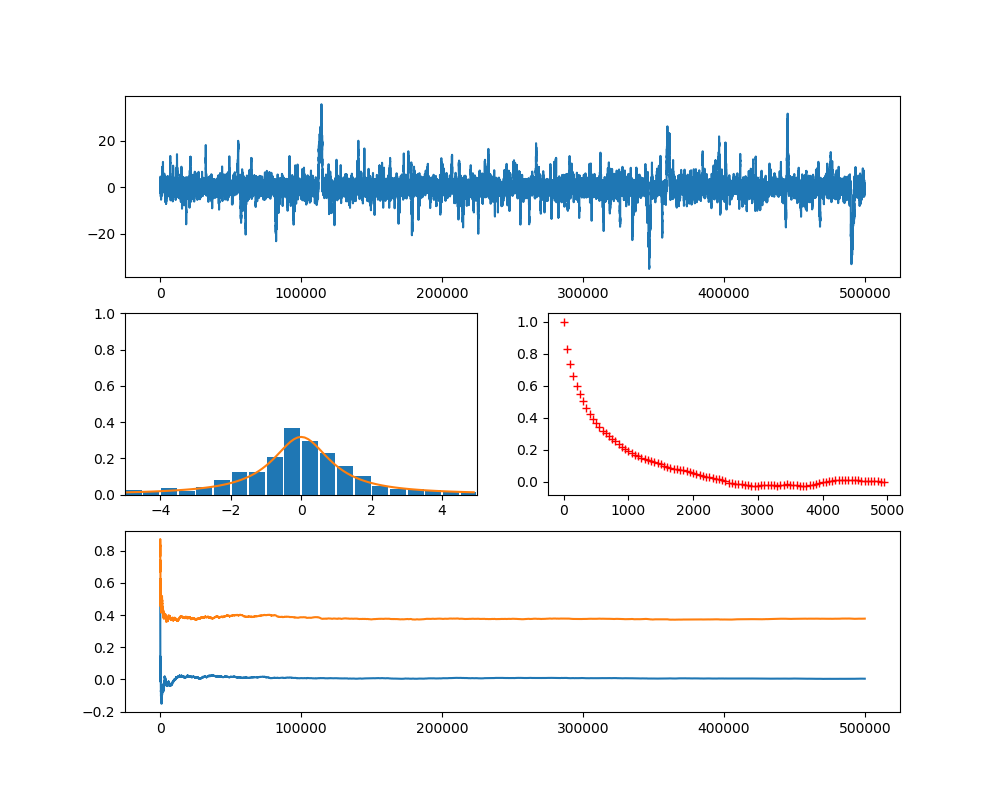
\includegraphics[scale=.45]{MetropolisCauchySample.png}

We see that after a few thousand steps, the chain converges, but continues to have spikes. However, the sampled distribution is very close to the sample generated by the Python standard method (which is to take the quotient of two
independent samples from a standard normal distribution). 

In the diagram at the bottom, we have displayed how the integral of two functions ($\sin(x)$ and $\cos(x)$) approximated using the partial sums develops over time. We see that even though we still have huge spikes, the integral remains comparatively stable and converges already after a few thousand iterations. Even if we run the simulation only for 1000 steps, we already get close to the actual values zero (for $\sin(x)$) and $\approx 0.3678$ (for 
$\cos(x)$, obtained using the \verb+scipy.integrate.quad+ integration routine).

In the second diagram in the middle row, we have plotted the {\em autocorrelation} versus the {\em lag}, as an indicator for the failure of the sample points to be independent. Recall that for two samples $X$ and $Y$, the Pearson correlation coefficient is the number
$$
\frac{E((X-\bar{X})(Y-\bar{(Y)})}{\sigma_X \sigma_Y}
$$
where $\sigma_X$ and $\sigma_Y$ are the standard deviations of $X$ and $Y$. In our case, given a lag, i.e. a number $l$ less than the length of the chain, we can form two samples, one consisting of the points $X_0, X_2, \dots$ and the second one consisting of the points of the shifted series $X_l, X_{l+1}, X_{l+2}, \dots$. The autocorrelation with lag $l$ is then defined as the correlation coefficient between these two series. In our diagram, we have shown how the autocorrelation depends on the lag. We see that for a large lag, the autocorrelation becomes small, supporting our intuition that the series and the shifted series become independent. However, if we execute several simulation runs, we will also find that in some cases, the convergence of the autocorrelation is very slow, so care needs to be taken when trying to obtain a nearly independent sample from the chain. Keep in mind that this is not the point of the Markov chain - the real point is that even though the sample is autocorrelated, we can approximate expectation values fairly well.

The Metropolis algorithm has used a symmetric proposal density, i.e. a density $q$ for which we have $q(x,y) = q(y,x)$. In fact, in the example above, the density was given by
$$
q(x,y) = q(|x-y|)
$$
and depends only on the distance between $x$ and $y$. Thus a Markov chain using $q$ without any additional accept/reject logic would be a random walk. Therefore this class of algorithms is sometimes called {\em random walk Metropolis}. 

A different subclass of the Metropolis-Hastings family of algorithms is obtained when we use proposal density that depends only on $y$, i.e.
$$
q(x,y) = q(y)
$$
In this case, the quantity $\alpha$ will be
$$
\alpha(x,y) = \min \{1, \frac{\pi(y) q(x)}{\pi(x) q(y)} \}
$$
This update rule is called an {\em independence sampler}. The quotient
$$
w(x) = \frac{\pi(x)}{q(x)}
$$
is called the {\em weight} function. With this, the acceptance probability can be written as
$$
\alpha(x,y) = \min \{1, \frac{w(y)}{w(x)} \}
$$
So we accept a new proposal preferred if its weight is not too small compared to the weight of the current step. 

It is interesting to compare this to an importance sampling with the density $q$. Recall that the idea behind importance sampling is to write an expectation value
with respect to $\pi$ as
$$
\int f \pi \lambda(dx) = \int f \frac{\pi}{q} q \lambda(dx) = 
\int (f \cdot w) q(dx)
$$
which is now an expectation value for the density $q$. This corresponds to weighting a sample point by $w$ in the approximation by the empirical mean of a sample. The difference is that for an ordinary importance sampler, we do not reject a proposal, which is allowed in a Metropolis-Hastings independence sampler.
 
Similar to an importance sampler, an independence sampler can behave very poorly
if the weight function has spikes or is not bounded. In fact, as we can see from the definition of $\alpha$, the chain easily gets stuck at points with a high weight. In addition, the algorithm easily gets numerically unstable as we divide by potentially small values $q(y)$. In general, independence sampling will only work if the proposal distribution has a similar shape as the target distribution and the weight function is bounded from below and from above (see also Theorem 6.3.1 in \cite{RobertCasella1999} for a more formal statement).

To illustrate how sensitive the independence sampler	 is with respect to the proposal distribution, the following diagrams - organized the same way as the illustration of the symmetric case - show to different simulations with the target distribution being an exponential distribution with mean value one. In the first simulation, we have chosen a normal distribution centered at one with standard deviation 10 as proposal distribution.

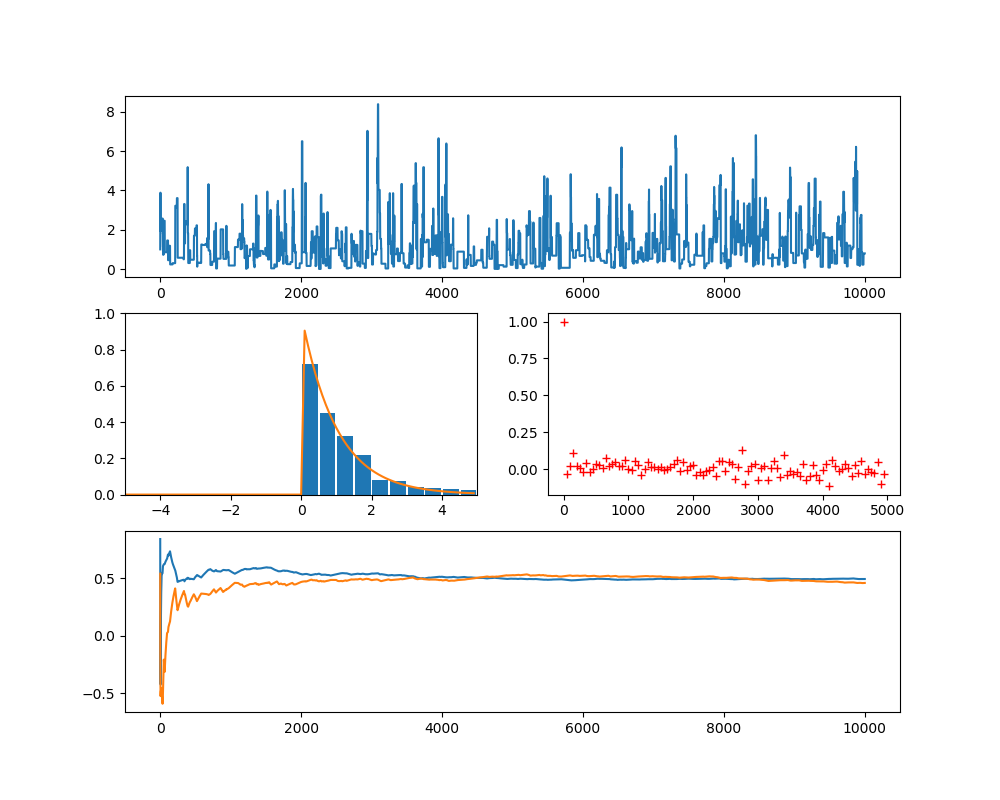
\includegraphics[scale=.45]{MetropolisIndependentGood.png}

The simulation was done with 10.000 steps, and we see that the result matches the target distribution rather well, even if we use every 10th point of the chain for the sample. We have also computed two integrals over the positive real axis ($\sin(x)$ and $\cos(x)$) which again converge quickly to their actual values (which is $0.5$ in both cases). We also see that the autocorrelation behaves nicely.

The following diagram shows the result of a similar simulation, the only difference being that this time, the standard deviation of the proposal distribution was $0.1$.

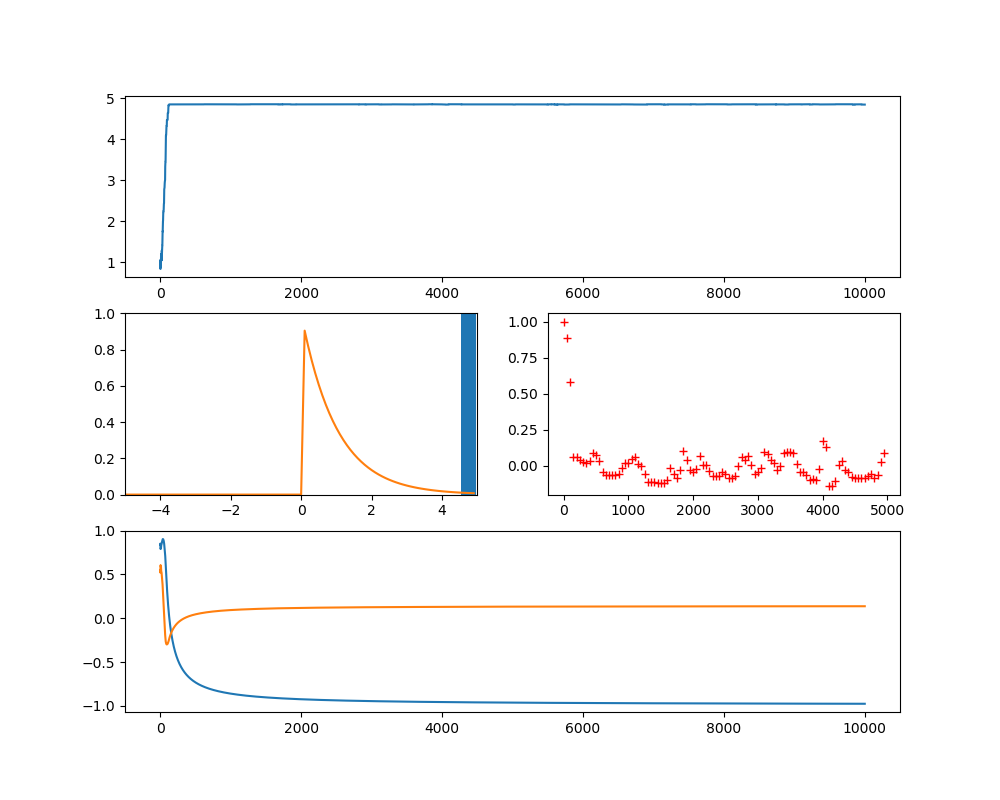
\includegraphics[scale=.45]{MetropolisIndependentBad.png}

Here we see that in fact, the chain quickly gets stuck at a value of $x$ close to 5 and never recovers from this situation. The resulting distribution as well as the integrals are grossly off the target, illustrating how badly an independence sampler can behave. The reason becomes clear if we look at the weight function, which is in fact finite but ridiculously large in most areas of the state space as the proposal density $q$ by which we divide has a very sharp peak (in fact, a straightforward implementation in Python will not even run without numerical overflows, and we have to cut off $q$ to make the program run at least technically correct, but as we see still with absurd results).

To close this chapter, let us quickly discuss under what conditions we can expect the algorithm to give meaningful results. Clearly, the Metropolis-Hastings algorithm works well only if the Markov chain behind it converges to the target distribution. From the previous chapter, we know that this happens if the chain is irreducible, aperiodic and recurrent. Intuitively, we expect the chain to be irreducible if the proposal density explores a sufficiently large region of the state space, i.e. if it is non-zero in some controllable region around the current location of the chain. Moreover, the fact that we can reject a proposal implies that the chain has a non-zero probability to stay where it is, which should guarantee that the chain is aperiodic. Finally, recurrence is a given as we already know that the chain has $\pi$ as an invariant distribution. Thus it is very likely that - except maybe in a few pathological case - the algorithm converges. This is in fact true, and we give a more precise argument in section \ref{sec:metropolishastingstheory}. We remark, however, that it is very hard to obtain bounds on the steps needed until convergence takes place, and this is the subject of ongoing and intensive research in this area. Our example for an independence sampler might serve as a warning illustrating this - theoretically, the chain does converge even with our bad choice for the proposal density (which has a very sharp spike, but is still non-negative, which makes the chain irreducible and recurrent), but convergence happens so slowly that the algorithm is useless in practice.

When sampling from high dimensional distributions, it is often more feasible to update one coordinate at a time, which is known as {\em variable-at-a-time} or {\em Gibbs within Metropolis} algorithm - this is in fact how the original algorithm in \cite{Metropolis1953} worked. In this version of the algorithm, our state space is a product
$$
{\mathcal X} = {\mathcal X}_1 \times \dots \times {\mathcal X}_d
$$
and we have $d$ potentially different proposal densities
$$
q_i \colon {\mathcal X} \times {\mathcal X}_i \rightarrow \R
$$
In each step, we pick some coordinate $i$ - we could do this by simply cycling through the coordinates $1, \dots d$ one by one or by choosing a coordinate at random with a uniform distribution. We then decompose the current location of the chain as
$$
x = (x_1, \dots, x_d)
$$
and draw a proposed new value $y_i$ for the $i$-th coordinate according to the distribution $q_i(x, \cdot)$. We then calculate an acceptance probability 
$$
\alpha(x,y_i) = 
\begin{cases}
\min \{ 1, \frac{\pi(y)q(y,x_i)}{\pi(x)q(x,y_i)} \} & \text{if } \pi(x) q(x,y_i) > 0 \\
1 & \text{if } \pi(x) q(x,y_i) = 0 
\end{cases}
$$
where 
$$
y = (x_1, \dots, x_{i-1}, y_i, x_{i+1}, \dots, x_d)
$$
We then accept the new location $y$ with probability $\alpha$ or reject it and stay at $x$. Then we proceed with the next coordinate.

Thus the variable-at-a-time algorithm works as the full Metropolis-Hastings algorithm, but successively applied to the individual coordinates. Of course the kernel given by one of the $q_i$ will not be irreducible, as it will only move along a hyperplane as it only changes coordinate $i$, but the combination of these kernels is in most cases again irreducible. It is also possible to prove regularity results for this algorithm to make sure that it converges, we refer the reader to \cite{RobertsRosenthal2006} or \cite{ChanGeyer1994} for some results in this direction and to \cite{Neal1993} for a short summary of the mathematical model (mixtures and cycles of Markov chains). 




\appendix


\section{Transition kernels}
\label{sec:transitionkernels}


For our study of markov chains, let us recall a few facts about transition kernels in general (see \cite{Klenke} chapter 14 or \cite{Bauer}, chapter 36 for the details). Suppose that $k_1$ is a finite kernel from $\Omega_1$ to $\Omega_2$ and $k_2$ is a finite kernel from $\Omega_2$ to $\Omega_3$. Then the assignment
$$
(\omega_1, A) \rightarrow \int {\mathbbm 1}_A (\omega_2, \omega_3) k_2(\omega_2, d\omega_3) k_1(\omega_1, d\omega_2)
$$
defines a kernel from $\Omega_1$ to $\Omega_2 \times \Omega_3$. Obviously,
$$
(k_1 \otimes k_2)(\omega_1, A_2 \times A_3) = \int k_1(\omega_1, d\omega_2) k_2(\omega_2, A_3)
$$
If $k_3$ is a third finite kernel from $\Omega_3$ to $\Omega_4$, we can consider $k_3$ equally well as a kernel on $\Omega_2 \times \Omega_3$ by ignoring the first factor, i.e. we extend
$$
k_3((\omega_2, \omega_3),A) =  k_3(\omega_3, A)
$$
Then we can iterate the construction and obtain a tensor product $k_1 \otimes k_2 \otimes k_3$ given by
$$
(k_1 \otimes k_2 \otimes k_3)(\omega_1, A) = \int {\mathbbm 1}_A k_3(\omega_3, d\omega_4)k_2(\omega_2, d\omega_3)k_1(\omega_1, d\omega_2)
$$
and so forth.

Let us now try to understand how these products are related to Markov chains. Given the data for a Markov chain as in definition \ref{defn:markovchain}, we can define a probability space ${\mathcal X}_0$ which consists of one point $*$ only and define a kernel $K_0$ from ${\mathcal X}_0$ to ${\mathcal X}$ by 
$$
K_0(\cdot, A) = \mu(A)
$$
where $\mu$ is the distribution of $X_0$ which we call the {\em initial distribution}. Thus
$$
K_0(*, A) = \mu(A) = P(X_0 \in A)
$$
Let us now compute the tensor product $K_0 \otimes K$. This is a kernel from ${\mathcal X}_0 = \{*\}$ to ${\mathcal X}  \times {\mathcal X}$. Unravelling the definition, we find that
$$
(K_0 \otimes K)(*, A) = \int {\mathbbm 1}_A \mu(dx_0) K(x_0, dx_1)
$$
To get used to the notation, let us spell out what exactly this means. For each $x_0$, we have a measure on ${\mathcal X}$ - given by $K(x_0, \cdot)$ - and a function on ${\mathcal X}$ - given by ${\mathbbm 1}_A(x_0, \cdot)$. We integrate this function over ${\mathcal X}$ using this measure and get a number. This procedure therefore defines a function of $x_0$. We then integrate this function using the measure $\mu$. Specifically, for $A = A_0 \times A_1$, we have
$$
(K_0 \otimes K)(x_0, A_0 \times A_1) = \int_{A_0} \mu(dx_0) K(x_0, A_1)
$$
Now this looks familiar. In fact, let us compute
\begin{align*}
P(X_1 \in A_1, X_0 \in A_0) &= \int_{X_0 \in A_0} {\mathbbm 1}_{X_1 \in A_1} dP \\
&= \int_{X_0 \in A_0} E({\mathbbm 1}_{X_1 \in A_1} | X_0) dP \\
&= \int_{X_0 \in A_0} P(X_1 \in A_1 | X_0) dP \\
&= \int_{A_0} P(X_1 \in A_1 | x_0) \mu(dx_0) \\
&= \int_{A_0} K(x_0, A_1) \mu(dx_0) \\
\end{align*}
which is the same expression. So we have shown that the joint probability of $X_0$ and $X_1$ is given by the measure $(K_0 \otimes K)(*)$:
$$
P_{X_0, X_1} = (K_0 \otimes K)(*)
$$
We can now easily iterate this argument. Let us compute the joint distribution of $X_2, X_1$ and $X_0$. We have
\begin{align*}
P(X_2 \in A_2, X_1 \in A_1, X_0 \in A_0) &= \int P(X_2 \in A_2 | x_0, x_1) dP_{X_0, X_1} \\
&= \int P(X_2 \in A_2 | x_1) dP_{X_0, X_1} \\
&= \int K(x_1, A_2) dP_{X_0, X_1} \\
&= \int K(x_1, A_2) K(x_0, dx_1) \mu(dx_0)
\end{align*}
If we translate this back into the language of tensor products, we find that
$$
P_{X_0, X_1, X_2} = (K_0 \otimes K \otimes K)(*)
$$
and so forth. Thus the joint distributions of the $X_i$ can be obtained as tensor products of the initial distribution with copies of the Markov kernel $K$. In particular, the initial distribution and the Markov kernel determine the joint distribution completely. 

Formally, the joint distribution is a distribution on the {\em sequence space}, which is the space ${\mathcal X}^{\Z_+}$ consisting of all sequences with values in${\mathcal X}$. It can in fact be shown that given a Markov transition kernel and initial distribution, we can construct a joint distribution on the sequence space as a projective limit, so that a Markov chain could alternatively be described as a distribution on a sequence space with certain properties. We will not need this point of view in these notes, but refer to \cite{Klenke}, Theorem 17.8 for the details.

Now let us turn our attention to the second type of composition that we can employ for Markov kernel. There are different ways to describe this composition. For our purpose, the easiest approach is via spaces of functions. Recall (see \cite{Bauer}, chapter 36) that a transition kernel $k$ from $\Omega_1$ to $\Omega_2$ can be described as a map
$$
k \colon E(\Omega_2) \rightarrow E(\Omega_1)
$$
where $E(\Omega_i)$ denotes the space of all non-negative measurable functions taking values in $\R_+ \cup \{+\infty\}$. Specifically, we set
$$
(kf)(\omega_1) = \int k(\omega_1, d\omega_2)f(\omega_2)
$$
A map of this type corresponds to a transition kernel if and only if it is additive, positive homogenous and has the property that whenever an increasing sequence of functions $f_n$ converges from below to $f$, then $kf_n \rightarrow kf$ from below.  Thus we can compose these maps and translate the result back into a transition kernel to define a product. If $k_1$ is a kernel from $\Omega_1$ to $\Omega_2$ and $k_2$ a kernel from $\Omega_2$ to $\Omega_3$, the resulting kernel from $\Omega_1$ to $\Omega_2$ (which is again Markov if this is true for $k_1$ and $k_2$) is given by
$$
(k_1 k_2)(\omega_1, A) = \int k(\omega_1, d\omega_2) k_2(\omega_2, A)
$$
Now let us again see how these products relate to Markov chains. First we compute the product $K_0 K$. For a function $f$ on ${\mathcal X}$, we have
$$
(K_0 Kf )(*) = \int \mu(dx_1) K(x_0, dx_1) f(x_1)
$$
where the integral is over $x_0$ and $x_1$. Applied to a characteristic function ${\mathbbm 1}_{A}$, we have
$$
(K_0 K)(*,A) = \int \mu(dx_0) K(x_0, A)
$$
So we see that again we can interpret this as a probability, namely as $P(X_1 \in A)$. Therefore we see that  the measure $(K_0 K)(*)$ is the distribution of $X_1$:
$$
P_{X_1} = (K_0 K)(*)
$$
What about higher powers? Let us write $K^n$ for the n-fold product of $K$ with itself. We can now almost guess the formula for $K_0 K^2$ applied to a function $f$:
$$
(K_0 K^2)(f)(*) = \int \mu(dx_0) K(x_0, dx_1) K(x_1, dx_2) f(x_2)
$$
In particular, for a characteristic function, we have
$$
(K_0 K^2)(*, A) = \int \mu(dx_0) K(x_0, dx_1) K(x_1, A) 
$$
On the other hand, we can compute the distribution of $X_2$ as follows:
\begin{align*}
P(X_2 \in A) &= \int P(X_2 \in A | x_1) dP_{X_1} \\
&= \int K(x_1, A_2) dP_{X_1} \\
&= \int K(x_1, A_2) K(x_0, dx_1) \mu(dx_0) 
\end{align*}
Thus we find that
$$
P_{X_2} = (K_0 K^2)(*)
$$
and so forth for higher powers. The same argument also shows that 
$$
P(X_n \in A | x_0 ) = K^n(x_0, A)
$$
as this is - by what we have seen above - the function that we need to integrate with respect to $\mu$ to obtain $P(X_n \in A)$, which is exactly the defining property for a version of the conditional probability. In other words, the $n$-fold power of the transition kernel measures the probability that starting at a point $x_0$, the process will have reached the set $A$ in step $n$. It is common to denote this conditional probability $P^n_{x_0}(A)$. As the chain is time homogenous, the probability to get from $x_m$ to a set $A$ in step $n+m$ is exactly the same, i.e. we could have done the same calculations with $X_s$ instead of $X_0$ for any index $s$.  For later reference, we summarize the relations that we have obtained so far.

\begin{lem}
	Suppose that $\{X_n\}$ is a Markov chain with Markov kernel $K$. Then the following relations hold.
	\begin{align}\label{lem:markovkernelproducts}
	P_{X_0, \dots, X_n} = (K_0 \otimes K \otimes \dots, K)(*) \\
	P_{X_n} = (K_0 K^n)(*) \\
	P(X_{n+s} \in A | X_s = x_s) = K^n(x_s, A) 
	\end{align}
\end{lem}
As we have defined $K^n$ as the $n$-fold product of a mapping with itself, it is obvious that
$$
K^{s+t} = K^s K^t
$$
i.e.
$$
K^{s+t}(x_0, A) = \int K^s(x_1, A) K^t(x_0, dx_1)
$$
These equations are called the {\em Chapman-Kolmogorov equations} and have a very appealing intuitive meaning: to the probability to get in $s+t$ steps from $x_0$ to a set $A$ is the weighted sum of the probabilities to get from any $x_1$ to $A$ in $s$ steps, weighted by the probability to be in $x_1$ after $t$ steps. 


\section{Irreducible Markov chains}\label{sec:irreduciblemarkovchains}

In this section, we explore the notion of irreducibility for Markov chains. To guide our intuition, we will start with the case of a finite state space.

\begin{defn}
	Given a finite Markov chain with kernel $K$, two states $i$ and $j$ are said to {\em communicate} if there exist numbers $n$ and $m$ (depending on $i$ and $j$) such that $K^n_{ij} > 0$ and $K^n_{ji} > 0$, i.e. if the state $i$ can be reached from $j$ with positive probability after a finite number of steps and vice versa. By convention, each state communicates with itself. 
\end{defn}

It is not difficult to see that this is an equivalence relation. In fact, is it clear from the definition that equivalence is symmetric and every state communicates with itself. Now suppose that $i$ communicates with $j$ and $j$ communicates with $k$. We want to show that $i$ communicates with $k$. By assumption, there are $n$ and $m$ such that 
$$
K^n_{ij} > 0
$$
and
$$
K^m_{jk} >0
$$
Now
$$
K^{m+n}_{ik} = \sum_s K^n_{is} K^m_{sk} \geq K^n_{ij} K^m{jk} > 0
$$
so we can reach $k$ from $i$. The same argument with $i$ and $k$ reversed shows that $i$ can be reached from $k$ and this shows transitivity. For a given state $i$, let $C(i)$ denote the equivalence class of $i$ under this relation. These classes are often called {\em communication classes}. If $i$ can be reached from $j$, i.e. if $K^n_{ij} > 0$ for some $n$, we will write $i \rightarrow j$. With this notation, $i$ and $j$ communicate if and only if $i \rightarrow j$ and $j \rightarrow i$.

\begin{defn}
	A Markov chain with finite state space ${\mathcal X}$ is called {\em irreducible} if there is a state $i$ such that $C(i) = {\mathcal X}$. 
\end{defn}

Thus an irreducible Markov chain is a Markov chain where every state can be reached by any other state in a finite number of steps.  

Why are irreducible Markov chains important? As the term already suggest, a general (finite) Markov chain can in a certain sense be split into a union of irreducible Markov chains. However, in general, a certain piece of the state space will remain. To state this decomposition, we need the following definition.

\begin{defn}
	Given a finite Markov chain, we say that an equivalence class $C(i)$ is {\em absorbing} if the chain will remain within $C(i)$ with probability one, i.e. if
	$$
	K(j,C(i)) = 1
	$$
	for every $j \in C(i)$
\end{defn}

Given a finite Markov chain, we can now split the state space into the equivalence classes $C(i)$. Suppose that we reorder the states such that the first few equivalence classes are exactly the absorbing classes and we also order the states by their equivalence class. Then the matrix $K$ will be as follows.
$$
K =
\begingroup % keep the change local
\renewcommand\arraystretch{1.5}
\begin{pmatrix}
\boxed{C_1} & &  & \\
& \boxed{C_2} & & \\
& & \boxed{C_3} & \\
\multicolumn{4}{c}{\framebox[100pt]{$D$}}
\end{pmatrix}
\endgroup
$$
Each of the subsets $C_i$ is absorbing, and hence the row sums in each of the $C_i$ are again one. Thus the $C_i$ are by themselves stochastic matrices and each of them defines a Markov chain. When discussing convergence, it turns out that only these matrices are relevant, as the part of the state space corresponding to the matrix $D$ is left with probability one. More precisely, we have (see for instance \cite{KemenySnell}, Theorem 3.1.1:

\begin{thm}
	Given a finite Markov chain, let $C$ denote the union of the absorbing communication classes of the chain. Then the probability that the chain will eventually reach a state in $C$ is one.
\end{thm}


\begin{proof}
	If $X_0$ is already in $C$, then the probability that it remains in $C$ is one by the definition of an absorbing communication class. So let us assume that $X_0 \notin C$. We claim that for every state $j$ in the complement of $C$, there is an $n > 0$ such that $K^n_{ji} > 0$ for some $i$ in $C$, i.e. that every state not in $C$ has a positive probability to reach $C$ after $n$ steps. 
	Before proving this claim, let us see why the theorem follows from it. If the chain has reached $C$ in step $n$, it will remain in $n$. As the state space is finite, we can therefore find an $n$ such that after $n$ steps, each state in the complement of $C$ can reach $C$ with a positive probability. Again using the fact that the state space is finite, we can therefore find a positive number $p$ such that each state in the complement of $C$ has reached $C$ after $n$ steps with probability at least $p$. Thus the probability that the chain still remains outside of $C$ after $n$ steps is $1 - p$. Applying the same argument to the new state after $n$ steps, we find that the probability that after $kn$ steps, the chain is still outside of $C$ is at most $(1-p)^k$. As $p > 0$, this number goes to zero as $k \rightarrow \infty$ and the result follows.
	
	We still have to show that for a given state $j \notin C$, we can find a $n$ such that $K^n_{ji} > 0$ for some $i \in C$. By assumption, the communicating class $C(j)$ is not absorbing. For that purpose, let us say that a communication class $A$ can be reached from a communication class $B$, denoted as $A \rightarrow B$, if there is a state $a \in A$ and a state $b \in B$ such that $a \rightarrow b$. As $A$ and $B$ are communication classes, every state in $A$ can be reached from any other state in $A$ and the same holds for $B$, so that $A \rightarrow B$ implies that any state in $B$ can be reached from any state in $A$. Therefore it is obvious that $A \rightarrow B$ and $B \rightarrow C$ is transitive. In addition, if $A \rightarrow B$ and $B \rightarrow A$, then $A = B$ as $A$ and $B$ are equivalence classes. Thus we can introduce a partial ordering on the set of communication classes by letting $A < B$ if $A$ can be reached from $B$. The minimal classes are then exactly the absorbing sets. If now $A$ is a non-absorbing communication class, it is non-minimal, hence we can find another communication class $B$ with $A \rightarrow B$. If $B$ is not yet absorbing, it is not minimal, so we can repeat this procedure to find a third communication class $C$ with $A \rightarrow B$ and $B \rightarrow C$, i.e. $A \rightarrow C$. If now $C$ is absorbing, we have demonstrated that from any state in $A$ we can reach a state in an absorbing class. If not, we can iterate the argument and will eventually arrive at a minimal and therefore absorbing class as the state space and therefore the number of classes is finite.
\end{proof}


In a general state space (again, general means that the $\sigma$-algebra of measurable sets in the state space is countably generated), the measure of a point will often be zero, and definitions that rely on the probability to reach an individual point do not make sense anymore. However, the idea remains the same as in the finite case - we are interested in chains where each sufficiently large set can be reached from any point. The idea of being sufficiently large can be made precise using a measure, which leads us to the following definition.

\begin{defn}
	Let $\{X_n\}$ be a Markov chain with state space ${\mathcal X}$ and let $\varphi$ be a non-trivial and $sigma-$finite measure on the $\sigma$-algebra of measurable sets in ${\mathcal X}$. We say that the chain is {\em $\varphi$-irreducible} and call $\varphi$ an {\em irreducibility measure} if, for every measurable set $A$ with $\varphi(A) > 0$ and every $x \in {\mathcal X}$, we can find some $n$ (depending on $x$ and $A$) such that
	$$
	K^n(x,A) > 0
	$$
\end{defn}

Note that we do not require that $\varphi$ be finite or a probability measure. This is in fact not a restriction. If $\varphi$ is any irreducibility measure, we can, as we assume $\varphi$ to be $\sigma$-finite, find an increasing sequence of sets $A_i$ with $\varphi(A_i) < \infty$ such that  
$$
{\mathcal X} = \bigcup_i A_i
$$
Now choose a sequence $a_k$ of non-negative numbers such that 
$$
a_k \leq 2^{-k}
$$
and
$$
a_k \varphi(A_k) \leq 2^{-k}
$$
We can now define a function $h$ by
$$
h = \sum_{n=1}^\infty a_n {\mathbbm 1}_{A_n}
$$
Then it is easy to show that $\int d \varphi(dx) \leq 1$. Further, $h$ is everywhere positive and bounded by one. Therefore 
$$
\varphi' = h \varphi
$$
is a finite measure with the same sets of measure zero as $\varphi$, and hence also $\varphi'$ is an irreducibility measure for our Markov chain, which we could scale to be a probability measure. We can therefore always assume that $\varphi$ is a probability measure and could have defined the notion of irreducibility only for probability measures (which is sometimes done, for instance in \cite{Revuz}, defn. 2.1).

There are a number of different formulations of irreducibility that are helpful to guide our intuition. To be able to state these conditions, let us introduce two more concepts. The first of these concepts is the occupation time.

\begin{defn}
	Given a measurable set $A \in {\mathcal X}$, the {\em occupation time} is the number
	$$
	\eta_A = \sum_{n=1}^\infty {\mathbbm 1}_{X_n \in A}
	$$
\end{defn}

Thus the occupation time counts how often a chain is in the set $A$. Note that, by its definition, this is a sum of random variables and therefore itself a random variable taking values in $\bar{R}_+$, i.e. the occupation time can be infinite. We will often be interested in the expectation value of the occupation time given a starting point $x$ and note for future reference that
$$
E_x(\eta_A) = E(\eta_A | X_0 = x) = \sum_{n=1}^\infty E({\mathbbm 1}_{X_n \in A} | X_0 = x) = \sum_{n=1}^\infty K^n(x,A)
$$
The occupation time measures how much time a process spends in a given set. In addition, it is often interesting to know when a chain enters a given set for the first time. 

\begin{defn}
	Given a measurable set $A$ in the state space, we define the {\em return time} of $A$ 
	$$
	\tau_A = \min\{ n \geq 1 | X_n \in A)
	$$
\end{defn}
Note that this is again a random variable. We also restrict the time to all times starting at one, so that if $X_0(\omega)$ is already in $A$, we really measure when the chain returns to $A$. After these preparations, we are now in a position to state and prove the following result.

\begin{lem}
	Suppose that $\{X_n\}$ is a Markov chain with state space ${\mathcal X}$. Given a measure $\varphi$ on ${\mathcal X}$, the following conditions are equivalent.
	\begin{enumerate}
		\item The chain is $\varphi$-irreducible
		\item For every set $A$ with $\varphi(A) > 0$ and every point $x$, we have 
		$$
		E_x(\eta_A) > 0
		$$
		\item For every set $A$ with $\varphi(A) > 0$ and every point $x$, we have 
		$$
		P_x(\tau_A < \infty) > 0
		$$
	\end{enumerate}
\end{lem}

\begin{proof}
	Let us first suppose that the chain is irreducible, and suppose that we are given a set $A$ with $\varphi(A) > 0$ and some starting point $x$. We then have
	\begin{align*}
	E_x(\eta_A) = \sum_{n=1}^\infty K^n(x,A)
	\end{align*}
	By the definition of irreducibility, we can find some $n$ such that $K^n(x,A) > 0$. Hence the expectation value is positive, and we have that $1 \Rightarrow 2$. Conversely,  if $E_x(\eta_A) > 0$, there must be at least one $n$ such that $K^n(x,A) > 0$, and this proves $2 \Rightarrow 1$. Thus we have shown the equivalence of condition 1 and condition 2.
	
	Next we will demonstrate that $3 \Rightarrow 2$. For that purpose, assume that we are given a measurable set $A$ and some starting point $x \in {\mathcal X}$. We then have the inequality
	\begin{align*}
	P_x(\tau_A = n) &= P_x(X_1 \notin A, X_2 \notin A, \dots, X_n \in A) \\
	& \leq P_x(X_n \in A) \\ &= K^n(x,A)
	\end{align*}
	and therefore
	\begin{align*}
	E_x(\eta_A) = \sum_{n=1}^\infty K^n(x,A) & \geq \sum_{n=1}^\infty  P_x(\tau_A = n) = P_x(\tau_A <\infty)
	\end{align*}
	which of course implies that $3 \Rightarrow 2$. To complete the proof, we only have to show that also $1 \Rightarrow 3$ holds. To see this, let us assume that the chain is irreducible, and let us try to express the event $X_n \in A$ in terms of the return times. Clearly,
	$$
	X_1 \in A \Leftrightarrow \tau_A = 1
	$$
	If $X_2 \in A$, we have to distinguish between two cases. Either the chain enters $A$ in the second step for the first time, i.e. $X_1 \in A$, or the chain already comes from a point in $A$. Thus
	\begin{align*}
	\{ X_2 \in A \} &= \{ \tau_A = 2 \} \cup \{ X_2 \in A, X_1 \in A \}   \\
	& = \{ \tau_A = 2 \} \cup  \{ X_2 \in A, \tau_A = 1 \}   \\
	\end{align*}
	and so forth. Taking conditional probabilities, we therefore see that
	$$
	K^n(x,A) = P_x(X_n \in A) = \sum_{k=1}^n P_x(X_n \in A, \tau_A = k) \leq \sum_{k=1}^n P_x(\tau_A = k)
	$$
	Thus if $K^n(x,A) > 0$, then for some $k$, we must have $P_x(\tau_A = k) > 0$, and therefore $P_x(\tau_A < \infty) > 0$ as claimed.
\end{proof}

\begin{example}
	Suppose that ${\mathcal X}$ is a finite state space with two elements $1$ and $2$. Consider the Markov chain given by the transition matrix
	$$
	K = \begin{pmatrix} 1 & 0 \\ p & 1 - p \end{pmatrix}
	$$
	with $p > 0$. Obviously, the state $1$ is absorbing and we have two communication classes which both contain only one state. it is possible to get from state 2 to state 1 with positive probability $p$, i.e. $2 \rightarrow 1$, but not $1 \rightarrow 2$. If we choose $\varphi$ to be the measure concentrated on $1$, then the chain is $\varphi$-irreducible. If we choose the counting measure that gives the same weight to both points, then the chain is not $\varphi$-irreducible. Thus in general, for a finite state space, the new concept of $\varphi$-irreducibility is weaker than that of irreducibility, and the measure $\varphi$ needs to be chosen carefully to be useful. Intuitively, the measure $\delta_1$ concentrated on one point is too small to fully capture the state space and needs to be extended. This leads to the notion of a maximal irreducibility measure.
\end{example}

We will now investigate how irreducibility depends on the measure $\varphi$. Recall that a measure $\varphi_1$ is called {\em absolutely continuous} with respect to a measure $\varphi_2$, written as $\varphi_1 \prec \varphi_2$, if $\varphi_2(A) = 0$ implies that $\varphi_1(A) = 0$. Two measures are called {\em equivalent} if they have the same sets of measure zero. 

\begin{defn}
	Suppose that $\{ X_n \}$ is a Markov chain with state space ${\mathcal X}$. We say that a measure $\psi$ on the state space is a {\em maximal irreducibility measure} if the chain is $\psi$-irreducible and for any other irreducibility measure $\varphi$, we have $\varphi \prec \psi$.
\end{defn}

\begin{prop}[see \cite{MeynTweedie} 4.22]\label{prop:maximalirreducibilitymeasure}
	If a Markov chain is $\varphi$-irreducible for some measure $\varphi$ on the state space, there is a probability measure $\psi$ which is a maximal irreducibility measure. This is given by
	$$
	A \mapsto \int \varphi'(dy) \sum_{n=0}^\infty K^n(y,A) 2^{-(n+1)}
	$$
	for any finite irreducibility measure $\varphi'$ where we set
	$$
	K^0(x,A) = {\mathbbm 1}_A(x)
	$$
	Any other maximal irreducibility measure is equivalent to this measure. 
	Further, if $\psi(A) = 0$, then $\psi(\{ y | P_y(\tau_A < \infty) > 0\}) = 0$
\end{prop}

Note that the measure $\psi$ is constructed in such a way that when a set $A$ can eventually be reached from a set with non-zero $\varphi$-measure, then $\psi(A)$ will be positive. In that sense, the measure is a sort of completion of $\varphi$. In particular, 
the last property implies that if $A$ has measure zero, then the set of all points $y$ from which we eventually reach $A$ also has measure zero. In other words, sets with measure zero are avoided from almost all starting points. 

It is common practice to reserve the letter $\psi$ for a maximal irreducibility measure. In that sense, we can make the following definition.


\begin{defn}
	A Markov chain is called {\em $\psi$-irreducible} if $\psi$ is a maximal irreducibility measure for the chain.
\end{defn}




\section{First entry and last exit decompositions}\label{sec:firstentrylastexit}

In this section, we briefly summarize a calculational tool related to Markov chains that is known as {\em first entry} and {\em last exit} decomposition. We start with a definition.

\begin{defn}
Given a Markov chain with transition kernel $K$ and measurable sets $A$ and $B$ in the state space, we call the number
$$
{_A}K^n(x,B) = P_x(X_n \in B, \tau_A \geq n)
$$
the {\em n-step taboo probability} for$A$ and $B$. Note that this is the probability that the chain reaches $B$ in step $n$, but avoids $A$ on the way to $B$. 
\end{defn}

It is not difficult to write down an explicit formula for the taboo probabilities. By using lemma \ref{lem:markovkernelproducts} and the definition of the tensor product of measures, we have
\begin{align*}
{_A} K^n(x,B) &= P_x(X_n \in B, \tau_A \geq n) \\
&=  P_x(X_n \in A, X_{n-1} \notin A^C, X_{n-2} \notin A^c, \dots) \\
&= \int_{A^c} K(x, dx_1) \int_{A^c} K(x_1, dx_2) \dots, \int_{A^c} K(x_{n-2}, dx_{n-1})
K(x_{n-1}, B) \\
&= \int_{A^c} K(x,dy) {_A}K^{n-1}(y,B)
\end{align*}
where we have recombined all integrals except the last one into an $(n-1)$-step taboo probability. As often, this is very intuitive - we take the integral over all possible ways to first get from the starting point $x$ to some small area $dy$ of the state space and then proceed from there to $B$ in n-1 steps without visiting $A$ first. Note that as a special case, we can set $A = B$ and obtain
$$
{_A}K^n(x,A) = P_x(X_n \in A, \tau_A \geq n) = P_x(\tau_A = n)
$$
and therefore obtain the recursion formula
$$
P_x(\tau_A = n) = \int_{A^c} K(x,dy) P_y(\tau_A = n-1)
$$
Following \cite{MeynTweedie}, let us introduce a few notations. First, we can consider the probability that a chain ever reaches a set $A$. This probability is denoted by $L(x,A)$, thus
$$
L(x,A) = P_x(\tau_A \geq \infty) = \sum_{n=1}^\infty P_x(\tau_A = n) = 
\sum_{n=1}^\infty {_A}K^n(x,A)
$$
More generally, we can consider the same sum for not necessarily identical sets $A$ and $B$. Thus we set
$$
{_A}U(x,B) = \sum_{n=1}^\infty {_A}K^n(x,B)
$$
so that
$$
L(x,A) = {_A}U(x,A)
$$
Now let us assume that we are given a set $B$ and some other set $A$. Then the sets
$$
B \cap \{\tau_A = 1\}, B \cap \{\tau_A = 2\}, \dots, B \cap \{ \tau_A = \infty \}
$$
form a partition of $B$ into disjoint subsets. Consequently, we can write
\begin{align*}
P^n(x,B) &= P_x(X^n \in B) \\
& = P_x(X_n \in B, \tau_A \geq n) + P_x(X_n \in B, \tau_A < n) 
\end{align*}
so that
$$
K^n(x,B) = {_A}K^n(x,B) + \sum_{k=1}^{n-1} P_x(X_n \in B, \tau_A = k) \\
$$
Let us try to express the second term as a sum of taboo probabilities as well. We have
\begin{align*}
P_x(X_n \in B, \tau_A = k) = &\int_{A^c} K(x,dx_1) \dots 
\int_A K(x_{k-1}, dx_k) \\
& \int_{\mathcal X} K(x_k, dx_{k+1}) \int_{\mathcal X}\dots K(x_{n-1}, B) \\
&= \int_{A^c} K(x,dx_1) \dots \int_A K(x_{k-1}, dx_k)   K^{n-k}(x_k, B) \\
&= \int_{A} {_A}K^k(x,dy) K^{n-k}(y, B)
\end{align*}
which proves the {\em first entry decomposition}
\begin{align}\label{eq:firstentrydecomposition}
K^n(x,B) = {_A}K^n(x,B) + \sum_{k=1}^{n-1} \int_{A} {_A}K^k(x,dy) K^{n-k}(y, B)
\end{align}
To obtain this decomposition, we have split the set of all chains that enter $A$ before step n according to the first entry time, i.e. we have decomposed the event
$$
\{ X_n \in B, \tau_A \leq n-1 \} =
\{ X_n \in B, X_1 \notin A, X_2 \notin A, \dots, X_{n-1} \notin A \}
$$
as
$$
\bigcup_{k=1}^{n-1} \{ X_n \in B,  X_k \in A, X_i \notin A \, \forall \, i < k \}
$$
However, there is a different decomposition of the same set that we could use and that splits the set according to the last time (less than $n$) the chain visits $A$, i.e.
$$
\{ X_n \in B, \tau_A \leq n-1 \} = 
\bigcup_{k=1}^{n-1} \{ X_n \in B,  X_k \in A, X_i \notin A \, \forall \, k < i \leq n-1 \}
$$
This gives us a different formula for the probability to reach $B$ in step n which is called the the {\em last exit decomposition}:
\begin{align}\label{eq:lastexitdecomposition}
K^n(x,B) = {_A}K^n(x,B) + \sum_{k=1}^{n-1} \int_{A} K^k(x, dy) {_A}K^{n-k}(y,B) 
\end{align}
For calculations, it is useful to express these formulas as an identity of formal power series. We therefore introduce the two power series in a variable $t$ given by
\begin{align*}
U^{(t)}(x,B) &= \sum_{n=1}^\infty K^n(x,B) t^n \\
{_A}U^{(t)}(x,B) &= \sum_{n=1}^\infty {_A}K^n(x,B) t^n
\end{align*}
Note that, as all coefficients are bounded by one, this can alternatively be interpreted as a
converging power series on $(-1,1)$ or on the open unit disc in the complex plane. If we let $t$ approach $1$ from the left, then the values are increasing and are thus either bounded (and then converging) or unbounded. In that sense the limits
$$
\lim_{t \rightarrow 1^-} U^{(t)}(x,B)
$$
and
$$
\lim_{t \rightarrow 1^-} {_A}U^{(t)}(x,B)
$$
exist, but can be $\infty$. In that sense
$$
L(x,A) = \lim_{t \rightarrow 1^-} {_A}U^{(t)}(x,A)
$$
and
$$
E_x(\eta_A) = \lim_{t \rightarrow 1^-} U^{(t)}(x,A)
$$
The first entry and the last exit decomposition can then be written as an identity of
power series, converging on $(-1,1)$, namely
\begin{align*}
U^{(t)}(x,B) &= {_A}U^{(t)}(x,B) + 
\int_{A} {_A}U^{(t)}(x,dy) U^{(t)}(y, B) \\
U^{(t)}(x,B) &= {_A}U^{(t)}(x,B) + 
\int_{A} U^{(t)}(x, dy) {_A}U^{(t)}(y,B) 
\end{align*}


\section{Periodic Markov chains}\label{sec:periodicmarkovchains}

In this section, we explore the notion of cycles and periodicity for Markov chains with general state spaces. We start with a definition.

\begin{defn}
	Given a Markov chain $\{ X_n \}$ with state space $\mathcal X$ which is $\psi$-irreducible and a natural number $d \geq 2$, a {\em d-cycle} is a collection $D_1, \dots, D_d$ of measurable subsets of ${\mathcal X}$ together with a measurable subset $N$ of ${\mathcal X}$ such that
	\begin{enumerate}
		\item The sets $D_i$ and $N$ form a partition of ${\mathcal X}$
		\item $\psi(N) = 0$
		\item For $x \in D_i$, $i < d$, we have
		$$
		K(x,D_{i+1}) = 1
		$$
		and if $x \in D_d$, we have
		$$
		K(x,D_1) = 1
		$$
		In other words, a chain will proceed to the subset $D_{i+1}$ after visiting $D_i$ and therefore cycle through the sets $D_1, \dots, D_d$ with probability one.
	\end{enumerate}
	We call the chain {\em aperiodic} if no such cycle exists.
\end{defn}

Let us see what we can say about the numbers $\psi(D_i)$ in the situation above. First, we claim that $\psi(D_i) > 0$ for all $i$. In fact, suppose that $\psi(D_{i+1}) = 0$ for some $i$ (where we include the case $i = d$ by letting $D_{d+1} = D_1$ to simplify our notation). Then, according to
proposition \ref{prop:maximalirreducibilitymeasure}, we have
$$
0 = \psi(\{ y | P_y(\tau_{D_{i+1}} < \infty) > 0 \}) 
$$
But for $y \in D_i$, the periodicity condition implies that
$$
P_y(\tau_{D_{i+1}} = 1) = 1
$$
and therefore
$$
D_i \subset \{ y | P_y(\tau_{D_{i+1}} < \infty) > 0 \}
$$
Thus we would be able to conclude that $\psi(D_i) = 0$ whenever $\psi(D_{i+1}) = 0$. Due to the fact that the $D_i$ together with $N$ form a partition of ${\mathcal X}$ and $\psi(N) = 0$, this would imply that $\psi({\mathcal X}) = 0$, a contradiction. Thus in fact all $D_i$ have positive measure with respect to $\psi$. 

It is tempting to assume that the numbers $\psi(D_i)$ are all equal, but it is easy to see that this is in general not the case. In fact, suppose that we have cycle $D_i$ with respect to some maximal irreducibility measure $\psi$. For any positive number $\alpha$, we can then define a measure
$\psi'$ by letting
\begin{align*}
\psi' | D_1 &= \frac{\alpha}{\alpha +1 } \psi | D_1 \\
\psi' | D_2 &= \frac{1}{\alpha +1 } \psi | D_2 \\
\end{align*}
and
\begin{align*}
\psi' | D_i &= \psi | D_i \, \, \text{for} \, \,  i \geq 3 \\
\psi' | N &= 0
\end{align*}
Then the measure $\psi'$ does clearly have the same sets of measure zero as $\psi$. Thus, the chain is irreducible with respect to $\psi'$ and $\psi'$ is a maximal irreducibility measure. Further, $\psi'$ is a probability measure if and only if $\psi$ is a probability measure. But, by construction
$$
\frac{\psi'(D_2)}{\psi'(D_1)} = \alpha \frac{\psi(D_2)}{\psi(D_1)}
$$
Thus we can realize any ratio between $\psi(D_1)$ and $\psi(D_2)$. In order to make sure that the sets $D_i$ have the same measure with respect to $\psi$, we therefore need an additional condition. One possible condition of this type is that $\psi$ be invariant, i.e. that $\psi K = \psi$. In fact, if 
$x \in D_i$, we have
$$
K(x, D_{i+1}) = 1
$$
where again we interpret $D_{d+1} = D_1$ and so forth, but if $x \notin D_i$, we have
$$
K(x,D_{i+1}) = 0
$$
Thus we can calculate
\begin{align*}
(\psi K)(D_{i+1}) &= \int_{\mathcal X} K(x,D_{i+1}) \psi(dx) \\
&= \int_{D_i} K(x,D_{i+1}) \psi(dx) \\
&= \int_{D_i} 1 \psi(dx) = \psi(D_i)
\end{align*}
and we obtain inductively that $\psi(D_i) = (\psi K^n)(D_{i+n})$. 
Thus if $\psi$ is invariant, this relation implies that $\psi(D_i) = \psi(D_j)$ for any two indices $i$ and $j$. 


\begin{example}\label{ex:aperiodintegrationkernel}
	Suppose that ${\mathcal X} = \R^n$ and the maximal irreducibility measure $\psi$ is absolutely continuous with respect to the Lebesgue measure. Let us consider a Markov kernel $K$ which is given by an non-negative integration kernel with respect to the Lebesgue measure, i.e. assume that
	$$
	K(x,A) = \int_A q(x,y) dy
	$$
	Assume further that $q$ is continuous and $q(x,x) > 0$ for all $x$. Thus a chain located at $x$ in step $n$ will stay in neighborhood of $x$ with positive probability. We claim that this implies that the chain is aperoidic.
	
	In fact, suppose that we given a d-cycle $D_i$ with $d \geq 2$.  The periodicity condition then implies that  if $x \in D_i$, some other set $D_j$ has volume one with respect to $K(x,\cdot)$, i.e. we have
	$$
	K(x,D_i) = 0
	$$
	for $x \in D_i$ and therefore
	$$
	0 = \int_{D_i} q(x,y) dy
	$$
	for every $x \in D_i$. 
	
	Now let us fix some index $i$. As $k$ is continuous and non-zero along the diagonal, we can, for any $x \in D_i$, find an open ball $B_x$ and some $\epsilon_x > 0$ such that $q(x,y) \geq \epsilon_x$ whenever $y \in B_x$. Then
	$$
	\epsilon_x \int_{D_i \cap B_x} dy \leq \int_{D_i \cap B_x} q(x,y) dy \leq \int_{D_i} q(x,y) dy = 0
	$$
	which implies that 
	$$
	\lambda(D_i \cap B_x) = \int_{D_i \cap B_x} dy = 0
	$$ 
	for every $x$, where $\lambda$ denotes the Lebesgue measure. As $\R^n$ is second countable, the open cover $\{B_x \}$ of $D_i$ has some countable subcover, i.e. we can find a countable set $A \subset X$ such that
	$$
	D_i = \bigcup_{x \in A} (D_i \cap B_x)
	$$
	Thus, we can conclude that $\lambda(D_i) = 0$ and consequently, as we did assume that $\psi$ is absolutely continous with respect to $\lambda$, that $\psi(D_i) = 0$. This is a contradiction, and hence no cycle can exist.
	
	Note that the above conclusion already holds if we only assume that the kernel is bounded from below by $q$, i.e. that there exists a continuous $q$, non-zero along the diagonal, such that
	$$
	K(x,A) \geq \int_A q(x,y) dy
	$$
\end{example}

\section{Transient and recurrent Markov chains}
\label{sec:transientandrecurrentmarkovchains}


In this section, we will study transient and recurrent Markov chains in general state space. Intuitively, a set is recurrent if the chain returns to this set infinitely often and transient if it leaves the set after finitely many iterations. We formalize these behaviours in the following definitions.

\begin{defn}
	A set $A$ is called {\em uniformly transient} if there is some $M > 0$ such that 
	$$
	E_x(\eta_A) \leq M
	$$
	for all $x \in \mathcal A$. A set is called {\em transient} if it can be covered by a countable collection of uniformly transient sets. A set $A$ is called {\em recurrent} if 
	$$
	E_x(\eta_A) = \infty
	$$
	for all $x \in A$. 
\end{defn}

We have characterized a transient set by a bound on $E_x(\eta_A)$ on the set $A$ itself. It turns out that this is equivalent to the existence of a bound on the entire state space. 

\begin{prop}\label{prop:transientimpliesboundedexpectation}
	If a set $A$ is transient, there exists a countable cover of $A$ by measurable sets $A_i$ and constants $M_i$ such that for all $x$ in the state space
	$$
	E_x(\eta_{A_i}) \leq M_i
	$$
\end{prop}

\begin{proof}
	By our previous definition, we can find a covering by sets $A_i$ and constants $N_i$ such that
	$$
	E_x(\eta_{A_i}) \leq N_i
	$$
	whenever $x \in A_i$. Now let us fix an index $i$ and consider the first entry decomposition
	$$
	U^{(t)}(x,A_i) = {_{A_i}}U^{(t)}(x,A_i) + 
	\int_{A_i} {_{A_i}}U^{(t)}(x,dy) U^{(t)}(y, A_i) 
	$$
	for an arbitrary point $x$ in the state space. In the integral on the right hand side, we have, as $y \in A_i$
	$$
	U^{(t)}(y, A_i) \leq U(y, A_i) = E_y(\eta_{A_i}) \leq N_i
	$$
	and therefore
	$$
	\int_{A_i} {_{A_i}}U^{(t)}(x,dy) U^{(t)}(y, A_i) 
	\leq N_i \int_{A_i} {_{A_i}}U^{(t)}(x,dy) = N_i {_{A_i}}U^{(t)}(x,A_i)
	$$
	We therefore obtain 
	$$
	U^{(t)}(x,A_i) \leq (1+N_i) U^{(t)}(x,A_i) \leq (1+N_i) L(x,A_i) \leq 1 + N_i
	$$
	Letting $t$ approach one from the left, we thus find that
	$$
	E_x(\eta_{A_i}) \leq 1 + N_i
	$$
	for all $x$. This shows our claim with $M_i = 1 + N_i$. 
\end{proof}

\begin{example}\label{ex:finitechainsarerecurrent}
	Every finite irreducible Markov chain is recurrent. To see this, consider an arbitrary set $A$ and pick some $i \in \mathcal A$ . Then
	$$
	E_i(\eta_A) = \sum_n K^n(i,A) = \sum_n \sum_{j \in A} K^n_{i,j} 
	$$
	If this row converges to a finite value, it follows in particular that the series 
	$$
	\sum_n K^n_{i,j}
	$$
	converges for every $i,j \in A$, so that $\lim_{n \rightarrow \infty} K^n_{i,j} = 0$ whenever $i,j \in A$. In particular, $K^n_{i,i}$ tends to zero as $n$ goes to $\infty$. Now pick any other point $u$ in the state space. Then, by the Chapman-Kolmogorov equations, we have
	$$
	K^{s+t}_{i,i} \geq K^s_{i,u} K^t_{u,i}
	$$
	As the chain is irreducible, we can find a $t$ such that $K^t_{u,i} > 0$. If we now let $s \rightarrow \infty$, the left hand side goes to zero. As $K^t_{u,i}$ is positive, this implies that
	$$
	\lim_{s \rightarrow \infty} K^s_{i,u} = 0
	$$
	As $u$ was arbitrary, the $i$-th row of the matrix $K^s$ tends to zero for large $s$. On the other hand, each $K^s$ is a stochastic matrix, i.e. the sum across the row $i$ is always one (intuitively, the chain has to be somewhere in the finite state space). This is a contradiction. 
\end{example}

From the definition above, it is far from obvious whether transient and recurrent sets can coexist in the same chain. It is one of the fundamental facts in the theory of Markov chain that this is not the case for irreducible chains. In fact, we have the following result (see \cite{MeynTweedie}, Theorem 8.0.1)

\begin{thm}
	Suppose that $\{ X_n \}$ is a $\psi$-irreducible Markov chain. Then either
	\begin{itemize}
		\item Every set $A$ with $\psi(A) > 0$ is recurrent (if this is the case, we say that the chain is recurrent), or
		\item The state space is transient (in this case, we say that the chain is transient)
	\end{itemize}
	So every irreducible chain is either recurrent or transient.
\end{thm}

\begin{proof}
	We restrict ourselves to the countable case which is far less technical and refer the reader to \cite{MeynTweedie}, chapter 8 for the general case. So let us suppose that ${\mathcal X}$ is countable and that the chain is irreducible with respect to the counting measure $\psi$. We say that a point $i$ is recurrent if the set $\{ i \}$ is recurrent, or, equivalently, if
	$$
	\sum_n K^n_{i,i} =  E_i(\eta_i) = \infty
	$$
	Now suppose that we can find one point $i$ which is recurrent. Then, by the Chapman-Kolmogorov equations, we have
	$$
	K^{n+s+t}_{u,v} \geq K^s_{u,i} K^n_{i,i} K^t_{i,v}
	$$
	and therefore
	$$
	\sum_n K^{n+s+t}_{u,v} \geq K^s_{u,i} (\sum_n K^n_{i,i}) K^t_{i,v}
	$$
	As the chain is irreducible, we can, for any two points $u,v$ in the state space, find $s$ and $t$ such that  $K^s_{u,i}$ and $K^t_{i,u}$ are positive. Then this relation implies that
	$$
	\sum_{n=1}^\infty K^{n+s+t}_{u,v} = \infty
	$$
	and therefore
	$$
	E_u(\eta_v) = \sum_n K^{n+s+t}_{u,v} = \infty
	$$
	Thus the assertion is proved once we can show that if no point in the state space is recurrent, the chain is transient. So let us assume that
	$$
	\sum_n K^n_{i,i} =  E_i(\eta_i) < \infty
	$$
	for every $i$. Then every point is transient. But as the state space is countable, this already provides a countable cover of the state space by transient sets and the state space is transient.
\end{proof}



Let us now turn to the question whether an invariant distribution exists for a Markov chain and how this relates to recurrence. We start by assuming the existence of an invariant distribution and explore its consequences. 

\begin{prop}\label{prop:invariantimpliesmaximal}
	Suppose that a Markov chain is $\varphi$-irreducible and $\pi$ is an non-trivial invariant measure. Then
	$\varphi \prec \pi$.
\end{prop}

\begin{proof}
	Consider the finite kernel $K_{\frac{1}{2}}$ given by
	$$
	K_{\frac{1}{2}} (x,A) = \sum_{n=0}^\infty 2^{-(n+1)} K^n(x,A)
	$$
	If $A$ is a measurable set such that $\varphi(A) > 0$, then, for every $x$, we can find an $n$ such that
	$$
	K^n(x,A) > 0
	$$
	by the definition of irreducibility. Consequently, if $\varphi(A) > 0$, then $K_{\frac{1}{2}}(x,A) > 0$ for all $x \in \{\mathcal X\}$. As $\pi$ is non-trivial, this implies that
	$$
	(\pi K_{\frac{1}{2}})(A) = \int K_{\frac{1}{2}}(x,A) \pi(dx) > 0 
	$$
	On the other hand, the invariance of $\pi$ implies that $\pi K^n = \pi$ for all $n \geq 0$ and therefore $\pi K_{\frac{1}{2}} = \pi$. We therefore see that $\pi(A) > 0$ as claimed.
\end{proof}

In what follows, we will simply say that the chain is $\pi$-irreducible in this situation, and the usage of the symbol $\pi$ will imply that the measure $\pi$ is invariant. 

A second but very fundamental observation is the following proposition, which also holds if the irreducibility measure itself is not invariant.

\begin{prop}\label{prop:positiveimpliesrecurrent}
	Suppose that a Markov chain is $\psi$-irreducible and admits a finite invariant distribution $\pi$. Then the chain is recurrent. Moreover, every transient set has zero measure with respect to $A$.
\end{prop}

\begin{proof}
	It is sufficient to show that the second statement is true, as we can apply it to ${\mathcal X}$ to arrive at a contradiction. So let $A$ be a transient set. We can then find a countable cover $A_i$ of $A$ and constants $M_i$ such that 
	$$
	E_x(\eta_{A_i}) = \sum_{n=1}^\infty K^n(x,A_i) \leq M_i
	$$
	for constants $M_i$ and all $x$. 
	Let us now consider one index $i$. We have
	$$
	\int_{{\mathcal X}} E_x(\eta_{A_i}) \pi(dx) \leq \pi({\mathcal X}) M_i
	$$
	On the other hand, we have
	\begin{align*}
	\int_{{\mathcal X}} E_x(\eta_{A_i}) \pi(dx)   
	&= \sum_{n=1}^\infty \int_{{\mathcal X}} \pi(dx) K^n(x,A_i) \\
	&= \sum_{n=1}^\infty \pi K^n(A_i) 
	= \sum_{n=1}^\infty \pi(A_i) \\
	\end{align*}
	where we have used the fact that $\pi$ is invariant. Combining this, we obtain
	$$
	M_i \pi({\mathcal X}) \geq \sum_{n=1}^\infty \pi(A_i)
	$$
	As $\pi({\mathcal X}) < \infty$, this is only possible if $\pi(A_i) = 0$. But as the $A_i$ form a countable cover of $A$, this implies that $\pi(A) = 0$ as claimed.
\end{proof}

Thus we can only hope to find a finite invariant measure if the chain is recurrent. It is custom to call these chains positive.

\begin{defn}
	A Markov chain is called {\em positive} or {\em positive recurrent} if it is $\psi$-irreducible and admits a finite invariant measure. 
\end{defn}

We have thus shown that positive recurrent chains are in fact recurrent, thus justifying the usage of the term positive recurrent. 

We remark that there is a different characterization of a positive chain which explain the usage of the term "positive" in this context. In fact, one can show (see \cite{MeynTweedie}, Theorem 18.2.2) that a $\psi$-irreducible chain is positive if and only if for every set $A$ with $\psi(A) > 0$, we have
$$
\lim \sup_{n \rightarrow \infty} P^n(x,A) > 0
$$
for all startings point $x \in A$. 

The following theorem is the main result about the existence of invariant measures. The proof is beyond the scope of this introduction, and we refer the reader to \cite{MeynTweedie} theorem 10.0.1 and section 10.4 for the details.

\begin{thm}
	Suppose that a Markov chain is $\psi$-irreducible and recurrent. Then there exists an invariant measure $\pi$. This measure is unique up to multiplication with a positive constant.
\end{thm}


\begin{example}
	Consider the random walk on $\R$, i.e.
	$$
	X_{n+1} = X_n + W_n
	$$
	where the $W_n$ are independent and equally distributed. Assume that $W$ is given by a continuous distribution function $\gamma$. Then the transition kernel is given by
	$$
	K(x,(a, b)) = P(a-x \leq W \leq b-x) = \int_{a-x}^{b-x} \gamma(t) dt = \int_a^b \gamma(t-x) dt
	$$
	Let $\lambda$ denote the Lebesgue measure and let us compute the product $\lambda K$. We have
	\begin{align*}
	(\lambda K)(a,b) & = \int_{\R}  K(x,(a,b)) dx  \\
	&= \int_{\R} dx \int_a^b \gamma(t-x) dt \\
	&= \int_a^b dt \int_{\R} \gamma(t-x) dx \\
	& = \int_a^b dt \int_{\R} \gamma(y) dy =  \int_a^b dt = b - a = \lambda((a,b))
	\end{align*}
	where we have used the translational invariance of the Lebesgue measure. Therefore we can conclude that $\lambda K = \lambda$ and thus the Lebesgue measure $\lambda$ is an invariant measure.  
	Now suppose further that $\gamma > 0$ everywhere. Then, if $A$ is a Lebesgue measurable set of positive measure, we have that
	$$
	K(x,A) = \int_A \gamma(t-x) dt > 0
	$$
	and therefore the chain is $\lambda$-irreducible. Hence it is $\psi$-irreducible for some $\psi$ with $\lambda \prec \psi$. On the other hand, we have seen that $\psi \prec \lambda$. Therefore $\psi$ is equivalent to $\lambda$. If moreover $\gamma(0) > 0$, we can argue as in example
	\ref{ex:aperiodintegrationkernel} that the chain is aperiodic. Thus we have a $\psi$-irreducible and aperiodic chain which has an invariant measure, but no finite invariant measure, hence the chain is not positive recurrent. 
	
	In fact, one can show (see \cite{MeynTweedie}, prop. 9.5.3, that if the expectation value of $W$ is positive, the chain is transient. Thus we have an example
	of a transient chain that admits an invariant distribution. If, however, the mean value is zero and the second moment of $W$ is finite, then the chain is recurrent (see \cite{MeynTweedie}, 
	prop. 9.4.5). This provides examples of Markov chains which are irreducible, aperiod and recurrent, but not positive recurrent. 
\end{example}

The last theorem in combination with the last example shows that the set of recurrent (and $\psi$-irreducible, which is always implicit when talking about recurrent chains) Markov chains can be split into two different classes. The first class consists of those chains for which the - unique up to a constant - invariant measure is finite, these chains are the {\em positive recurrent} chains. The other class consists of those chains for which no finite invariant measure exists, i.e. every invariant measure is infinite. These chains are called {\em null recurrent}.

In the applications we are interested in, namely Markov chain Monte Carlo methods, one usually starts with a given measure $\pi$ and tries to construct a Markov chain which has $\pi$ as an invariant measure. Thus we know from the beginning whether this chain will be positive recurrent or null recurrent. 


\section{Total variation of measures}\label{sec:totalvariationnorm}

In this section, we assemble a few facts about the total variation norm of a measure.

\begin{prop}
	For a signed measure $\mu$ on a measurable space ${\mathcal X}$, we have the equality
	$$
	\| \mu \|_{TV} = \sup \{  \int f d\mu \, | \, f \in L^\infty({\mathcal X}) \, , \, |f| \leq 1   \}
	$$
\end{prop}

\begin{proof}
	First let us assume that we are given some measurable function $f$ with $|f| \leq 1$. We want to show that $\int f d\mu \leq \| \mu \|_{TV}$. This is obvious if the integral is negative, as the total variation norm is clearly a non-negative number, so we can assume that 
	$$
	\int f d\mu \geq 0
	$$
	Let us consider the sets
	$$
	A^+ = \{ f \geq 0 \}
	$$
	and 
	$$
	A^- = \{ f < 0 \} = {\mathcal X} - A^+
	$$
	If we set 
	$$
	f^+ = {\mathbbm 1}_{A^+} f 
	$$
	and
	$$
	f^- = - {\mathbbm 1}_{A^-} f 
	$$
	then
	$$
	f = f^+ - f^-
	$$
	and $f^+, f^- \geq 0$. 
	Now, by the Hahn decomposition theorem, we can find a partition of ${\mathcal X}$ into two disjoint measurable sets
	$$
	{\mathcal X} = {\mathcal X}^+ \cup {\mathcal X}^-
	$$
	such that $\mu$ is non-negative on ${\mathcal X}^+$ and non-positive on 
	${\mathcal X}^-$. Then
	$$
	\int f d\mu = \int_{A^+ \cap {\mathcal X}^+} f^+ d\mu  +
	\int_{A^+ \cap {\mathcal X}^-} f^+  d\mu
	+ \int_{A^- \cap {\mathcal X}^+} - f^- d\mu  
	+ \int_{A^- \cap {\mathcal X}^-} - f^- d\mu 
	$$
	The second and the third term are non-positive numbers. So we obtain
	$$
	\int f d\mu \leq \int_{A^+ \cap {\mathcal X}^+} f^+ d\mu  +  \int_{A^- \cap {\mathcal X}^-} - f^- d\mu 
	$$
	which we can estimate further (as $|f| \leq 1$) by
	$$
	\int f d\mu \leq  \mu(A^+) - \mu(A^-) = \mu(A^+) - \mu({\mathcal X} - A^+)
	$$
	Thus we obtain that 
	$$
	\int f d\mu \leq \| \mu \|_{TV}
	$$
	To show the converse, suppose that we are given a set $A$. Consider the function 
	$$
	f = {\mathbbm 1}_A - {\mathbbm 1}_{{\mathcal X} - A}
	$$
	Then $f$ is measurable and $|f| \leq 1$. Thus
	$$
	\mu(A) - \mu({\mathcal X} - A) = \int f d\mu \leq \sup \{  \int f d\mu \, | \, f \in L^\infty({\mathcal X}) \, , \, |f| \leq 1   \}
	$$
	and we obtain 
	$$
	\| \mu \|_{TV} \leq \sup \{  \int f d\mu \, | \, f \in L^\infty({\mathcal X}) \, , \, |f| \leq 1   \}
	$$
\end{proof}

Given two probability measures $\mu, \nu$, we can now form the total variation of their difference. Using 
$$
\mu({\mathcal X} - A) = 1 - \mu(A)
$$
and similarly for $\nu$, we find, using that the supremum is of course positive because we can always exchange $A$ with its complement, that
$$
\| \mu - \nu \|_{TV} = 2 \sup_{A} |\mu(A) - \nu(A)|
$$
Some authors define the total variation distance between two probability measures this way, dropping the factor of two. Finally, there is a third characterization of the total variation which is sometimes used.

\begin{prop}
	If $\mu$ is a signed measure on some measure space ${\mathcal X}$, then
	$$
	\| \mu \|_{TV} = \sup_{\{A_i\}} \sum_i | \mu(A_i) |
	$$
	where the supremum is taken over all countable partitions of ${\mathcal X}$ into
	measurable subsets $A_i$.
\end{prop}

\begin{proof}
	Let us suppose that we are given a partition into sets $A_i$. Note that it is a part of
	the definition of a signed measure that in the equality
	$$
	\mu({\mathcal X}) = \sum_i \mu(A_i)
	$$
	we can reorder the components arbitrarily, thus the sum converges absolutely and the sum
	$$
	\sum_i |\mu(A_i)|
	$$
	is finite. Let $I$ denote the set of indices for which $\mu(A_i) \geq 0$. Let
	$$
	A = \cup_{i \in I} A_i
	$$
	Then we have
	\begin{align*}
	\sum_i |\mu(A_i)| &= \sum_{\mu(A_i) \geq 0} \mu(A_i) - \sum_{\mu(A_i) < 0} \mu(A_i) \\
	&= \mu(A) - \mu({\mathcal X} - A) \leq \| \mu \|_{TV}
	\end{align*}
	On the other hand, if $A$ is some arbitrary measurable subset, then $A$ and 
	${\mathcal X} - A$ form a partition. We therefore have
	$$
	\mu(A) - \mu({\mathcal X} - A) \leq |\mu(A) - \mu({\mathcal X} - A)|
	\leq |\mu(A)| +  |\mu({\mathcal X} - A)| 
	\leq \sup_{\{A_i\}} \sum_i | \mu(A_i) |
	$$
	and hence
	$$
	\| \mu \|_{TV} \leq \sup_{\{A_i\}} \sum_i | \mu(A_i) |
	$$
	which completes the proof.
\end{proof}

It is not obvious from the definition, but can be shown (see for instance \cite{Rudin}, Theorem 6.4) that the total variation of any signed measure is finite. In addition, if $\mu$ and $\nu$ are signed measures, and $f$ is a measurable function bounded by one, we have
$$
\int f d(\mu + \nu) = \int f d\mu + \int f d_nu \leq \| \mu \|_{TV} + \| \nu \|_{TV}
$$
which implies the triangle inequality. Thus the space of signed measures is turned into a normed linear space by the total variation norm.

Let us briefly investigate the relation between the total variation norm and the concept of weak convergence. Recall that a sequence $\mu_n$ of finite measures is said to converge weakly to a finite measure $\mu$ if for all continuous and bounded functions $f$, we have
$$
\lim_{n \rightarrow \infty} \int f d\mu_n = \int f d\mu
$$
Of course this definition only makes sense if the space ${\mathcal X}$ carries a topology, so that
we can talk about continuous functions.Now it turns out that convergence in the total variation norm implies weak convergence. In fact, suppose that the measures $\mu_n$ converges to $\mu$ in total variation, i.e. that
$$
\lim_{n \rightarrow \infty} \| \mu_n - \mu | = 0
$$
Then, given a continuous function $f$ bounded by $C$, we have
$$
\int f d\mu_n - \int f d\mu = C \int \frac{1}{C} f d(\mu_n - \mu) \leq \| \mu_n - \mu \|_{TV} \rightarrow 0
$$
and thus we have weak convergence. Thus convergence in total variation is stronger than weak convergence and has the additional advantage that is can be formulated without a topology on the space ${\mathcal X}$.

\section{Harris recurrence}\label{sec:harrisrecurrence}

To introduce this concept, let us first recall that for every set $A$, we can define the number
$$
L(x,A) = P_x(\tau_A < \infty) 
$$
which is the probability that the chain ever visits $A$ starting at $x$. If we are given some point $x \in A$ and $\psi(A) > 0$, and we know that the chain is recurrent, then we know that the expectation value 
$$
U(x,A) = E_x(\eta_A) = \infty
$$
i.e. the expected number of visits of the set $A$ is infinite. How are these two quantities related to each other?
First, suppose that we have a set $A$ such that 
$$
L(x,A) = 1
$$
for all $x \in A$, i.e. if we ever reach $A$, we will return in a finite time with probability one. We can then write down the last exit decomposition for this set (see 
appendix \ref{sec:firstentrylastexit}) and obtain
$$
U^{(t)}(x,A) = {_A}U^{(t)}(x,A) + \int_A U^{(t)}(x,dy){_A}U^{(t)}(y,A)
$$
If we let $t \rightarrow 1^-$, then ${_A}U^{(t)}(y,A)$ will approach $L(y,A)=1$ for every
point $y \in A$. Hence we obtain that
$$
U(x,A) = L(x,A) + U(x,A) = 1 + U(x,A)
$$
for every $x \in A$. This is only possible if $U(x,A) = \infty$, thus the set $A$ is recurrent. Let us now make the following

\begin{defn}
	A set $A$ is called {\em Harris recurrent} if 
	$$
	L(x,A) = P_x(\tau_A < \infty) = 1
	$$
	for every $x \in A$. We call a Markov chain Harris recurrent if it is $\psi$-irreducible
	and every set $A$ with $\psi(A) > 0$ is Harris recurrent. The chain is called {\em positive Harris} if it is Harris recurrent and positive recurrent.
	
\end{defn}

Our calculation then shows that Harris recurrence implies recurrence, i.e. a set which is Harris recurrent is recurrent, and a Harris recurrent chain is recurrent. Now it turns out that Harris recurrence is what we need to prove strong convergence results. The key result which is sometimes called the {\em ergodic theorem} for Markov chains is as follows.

\begin{thm}[Ergodic theorem,see for instance \cite{MeynTweedie}, 13.3.3]
	If a Markov chain with transition kernel $K$ is aperiodic and positive Harris with finite invariant measure $\pi$, then for every 
	initial distribution $\mu$, 
	$$
	\lim_{n \rightarrow \infty} \| \int \mu(dx)K^n(x, \cdot) - \pi(\cdot) \|_{TV} = 0
	$$
\end{thm}


The proof is very technical and beyond our scope, we refer the reader to \cite{MeynTweedie}, chapter 13 for a proof. We remark that the choice $\mu = \delta_x$ for some point $x$ in the state
space immediately gives
$$
\| K^n(x,\cdot) - \pi(\cdot) \|_{TV} \rightarrow 0
$$
when $n$ tends to infinity. In particular, given a measurable set $A$, we have
$$
\lim_{n \rightarrow \infty} P_x(X_n \in A) = \pi(A)
$$

In addition to this result which states that the measures $K^n$ converge, we also have a version of the law of large numbers, which states that the expectation value of a function can be approximated by the empirical mean of a sample provided by a Markov chain - even though the $X_n$ are of course not independent and not identically distributed.

\begin{thm}[see for instance \cite{MeynTweedie}, Theorem 17.1.7]
	If a Markov chain is positive Harris with finite invariant measure $\pi$, then, for each measurable function $f$ on the state space which is integrable with respect to $\pi$ and every starting point $x$, the law of large numbers holds, i.e.
	$$
	\lim_{n \rightarrow \infty} \frac{1}{n} \sum_{k=1}^n f(X_n) = \int f d\pi 
	\qquad \text{a.s. } P_x 
	$$
\end{thm}

Note that the measure $P_x$, for a given starting point $x$, is to be interpreted as a measure on the sequence space ${\mathcal X}^\N$ to make sense out of this, and similarly the function $f(X_n)$ is to be interpreted as a function on that space, i.e. the composition of $f$ with the projection on the $n$-th coordinate.

Thus we see that positive Harris chains do in fact have very strong convergence properties. This raises the question whether every recurrent chain is in fact Harris recurrent. The answer is no, but fortunately it still turns out that every recurrent chain is in a certain sense Harris recurrent  - we can in fact turn every recurrent Markov chain into a Harris recurrent chain by splitting off a transient set of measure zero. 

\begin{thm}[\cite{MeynTweedie}, Theorem 9.0.1 and Theorem 9.1.5]
	\label{thm:maximalharrisset}
	Given a $\psi$-irreducible and recurrent Markov chain on the state space ${\mathcal X}$, there is a partition
	$$
	{\mathcal X} = N \cup H
	$$
	where $H$ is absorbing, every subset of $H$ with non-zero $\psi$-measure is Harris recurrent, $\psi(N)=0$ and $N$ is transient. Moreover, the set $H$ can be chosen to be {\em maximal absorbing}, i.e. if for some point $x$
	$$
	P_x \{\tau_H < \infty \} = 1
	$$
	then $x \in H$. 
\end{thm}

In particular, every finite recurrent chain and every recurrent chain on a countable state space is automatically Harris recurrent. For general chains, many results on Harris chains can be carried over to recurrent chains outside of a set of measure zero. As an example, consider the following corollary. 

\begin{cor}[13.3.4 in \cite{MeynTweedie}]
	Given a positive recurrent and aperiodic Markov chain with invariant measure $\pi$, there is a set $N$ with $\pi(N) = 0$ such that 
	$$
	\lim_{n \rightarrow \infty} \| \int \mu(dx)K^n(x, \cdot) - \pi(\cdot) \|_{TV} = 0
	$$
	for every initial distribution $\mu$ with $\mu(N)=0$. 
\end{cor}

\begin{proof}
	As the chain is recurrent, we can find a decomposition 
	$$
	{\mathcal X} = H \cup N
	$$	
	such that $H$ is absorbing, $\psi(N)=0$, $N$ is transient and such that every set $A \subset H$ with $\psi(A) > 0$ is Harris recurrent. As $H$ is absorbing, we have
	$$
	K(x,H) = 1
	$$
	for every $x \in H$. We can thus restrict $K$ to $H$ to define a Markov transition kernel for the state space $H$. As $\psi(N) = 0$, it is easy to see that $\psi$ again defines a maximal irreducibility measure for the Markov chain on $H$ defined by this kernel. Now $N$ is transient, and therefore $\pi(N) = 0$ by proposition \ref{prop:positiveimpliesrecurrent}. Hence we can restrict $\pi$ to $H$ to obtain a positive invariant
	measure for the chain on $H$. It is also not difficult to see that the new chain is aperiodic, as the definition of a cycle is modulo sets of measure zero. If now $\mu$ is any initial distribution with $\mu(N) = 0$, this defines an initial distribution on $H$ and we can apply the ergodic theorem to see that
	$$
	\lim_{n \rightarrow \infty} \| \int_H \mu(dx)K^n(x, \cdot) - \pi(\cdot) \|_{TV} = 0
	$$
	as an identify of measures on $H$. As $K^n(x,H) = 1$ for all $x \in H$, we have that
	$$
	K^n(x,N) = 0
	$$
	for all $x \in H$ and therefore the same identity holds as an identity of measures on 
	${\mathcal X}$. Finally, we can extend the integral to ${\mathcal X}$ as $N$ has measure zero with respect to $\mu$.
\end{proof}

Similarly, one can show that the law of large numbers holds for $\pi$-almost all starting points if the chain is positive recurrent. 

\begin{cor}
	If a Markov chain is positive recurrent with finite invariant measure $\pi$, and $f$ measurable and integrable with respect to $\pi$, then, for almost all starting points $x$, we have
	$$
	\lim_{n \rightarrow \infty} \frac{1}{n} \sum_{k=1}^n f(X_n) = \int f d\pi 
	\qquad \text{a.s.} P_x
	$$
\end{cor}

\section{Metropolis Hastings kernel}
\label{sec:metropolishastingstheory}

In this section, we assemble some of the theoretical results behind the Metropolis-Hastings algorithm. Recall that the algorithm works as follows.

We are given a target density $\pi$ from which we want to draw samples. We do this by choosing a proposal density $q(x,y)$ from which we can draw samples easily. For any two points $x,y$, we define
$$
\alpha(x,y) = 
\begin{cases}
\min \{ 1, \frac{\pi(y)q(y,x)}{\pi(x)q(x,y)} \} & \text{if } \pi(x) q(x,y) > 0 \\
1 & \text{if } \pi(x) q(x,y) = 0 
\end{cases}
$$
We now simulate a Markov chain as follows. We start with some arbitrary point $x_0$. When the chain 
has arrived at $x_n$, we first generate a candidate $y$ for the next location from the 
distribution $Q(x_n, \cdot)$. We now calculate $\alpha = \alpha(x_n, y)$. We then accept the proposal with probability $\alpha$, i.e. we draw a random sample $U$ from a uniform distribution
and accept if $U \leq \alpha$. If the proposal is accepted, we set $x_{n+1} = y$, otherwise we set
$x_{n+1} = x_n$.

Let us try to translate this algorithm into a theoretical model. First, we want to write down the Markov kernel driving this chain.
Given a region $A$ in the state space, we want to calculate the probability that, given that step $X_n$ is a point $x$, we reach $A$ in step $n+1$. By construction, the conditional probability to accept a proposal conditioned on the value $y$ of the proposal is
$$
\alpha(x,y)
$$
Therefore the probability to accept a proposal in the region $A$ is
$$
\int_A q(x,y) \alpha(x,y)
$$
and the overall probability to accept the next proposal is
$$
\alpha(x) = \int_{\mathcal X} q(x,y) \alpha(x,y)
$$
If we let $\delta_x$ denote the probability measure with support $\{ x \}$, and let
$$
r(x) = 1 - \alpha(x)
$$
denote the probability for rejection, we therefore have
$$
K(x,A) = \int_A q(x,y) \alpha(x,y) + r(x) \delta_x(A)
$$
for the probability to reach the region $A$. Here the first term is the probability that we accept and move to $A$, and the second term is the probability that we reject and end up in $A$ (which is of course only possible if $x \in A$). This motivates the following formal definition.


\begin{defn}
	Suppose that ${\mathcal X}$ is an open subset of $\R^n$ and that $\pi$ is a continuous probability density on $\R^n$ which is nowhere zero on ${\mathcal X}$. Suppose further that $q(x,y)$ is a finite, measurable and non-negative function on ${\mathcal X} \times {\mathcal X}$ such that
	$$
	\int q(x,y) \lambda(dy) = 1
	$$
	for all points $x$, where $\lambda$ is the Lebesgue measure on $\R^n$, i.e. that $q(x,\cdot)$ defines a probability measure on ${\mathcal X}$ for each $x$. 
	Define $\alpha(x,y)$ by
	\begin{align}\label{eq:metropolishastingsacceptanceprobability}
	\alpha(x,y) = 
	\begin{cases}
	\min \{ 1, \frac{\pi(y)q(y,x)}{\pi(x)q(x,y)} \} & \text{if } \pi(x) q(x,y) > 0 \\
	1 & \text{if } \pi(x) q(x,y) = 0 
	\end{cases}
	\end{align}
	and let
	$$
	r(x) = \int_{\mathcal X} q(x,y) \alpha(x,y) \lambda(dy)
	$$
	Then the Markov kernel 
	\begin{align}\label{eq:metropolishastingskernel}
	K(x,A) = \int_A q(x,y) \alpha(x,y) \lambda(dy) + r(x) \delta_x(A)
	\end{align}
	is called the {\em Metropolis-Hastings kernel} for the {\em target density} $\pi$ and the {\em proposal density} $q$. 
\end{defn}

We have assumed that the state space ${\mathcal X}$ is open (which is not really essential, but simplifies a few arguments) and contained in the support of $\pi$. This is not overly restrictive, as we typically start a simulation with a value $x$ for which $\pi(x) > 0$ and then the update rule will make sure that a proposal $y$ with $\pi(y) = 0$ is rejected almost surely. Therefore the simulated chain will never leave the support of $\pi$. We also restrict ourselves to continuous target densities, even though discrete versions are of course possible, and it is not difficult to adjust our arguments to the discrete case. We do, however, not assume that $q$ be continuous, as this would exclude some possible proposal densities like the uniform distribution that we might want to use in practice.

Before we investigate the properties of this kernel further, let us introduce the concept of a reversible chain.

\begin{defn}
	Suppose that a Markov chain with transition kernel $K$ is given by a density $k(x,y)$ with respect to some dominating measure $\lambda$ and that $\pi$ is a probability density with respect to $\lambda$. We call the chain {\em reversible} if for any two points $x, y$
	$$
	\pi(x) k(x,y) = \pi(y) k(y,x)
	$$
\end{defn}

It is not difficult to see that if the chain starts in $\pi$ in this situation, the joint distribution of $(X_0, X_1, \dots X_n)$ is the same as that of $(X_n, X_{n-1}, \dots,X_0)$ for any $n$. Thus the chain looks the same when we go backward in time. Another interpretation is that if the chain is in state $\pi$, then $\pi(x) k(x,y)$ is the number of sample paths that move from $x$ to $y$ in a given step, whereas $\pi(y) k(y,x)$ is the number of sample moving from $y$ to $x$, so the equality implies that the number of sample paths that are in $x$ and $y$ is constant over time. In fact, in this situation, $\pi$ is automatically a stationary distribution:
\begin{align*}
(\pi K)(A) &= \int \pi(x) K(x,A) \lambda(dx)  \\
&= \int_{\mathcal X} \lambda(dx) \int_A \lambda(dy) \pi(x) k(x,y)   \\
&= \int_{\mathcal X} \lambda(dx) \int_A \lambda(dy) \pi(y) k(y,x)    \\
&= \int_A \lambda(dy) \pi(y)  \int_{\mathcal X} \lambda(dx)  k(y,x)  = \int_A \lambda(dy) \pi(y) 
= \pi(A)
\end{align*}


We now note that the kernel given by $q(x,y) \alpha(x,y)$ has a similar property. In fact, it immediately follows from the definition of $\alpha$ that
\begin{align}
\pi(x) \alpha(x,y) q(x,y) = \min \{ \pi(x) q(x,y), \pi(y) q(y,x)  \}
\end{align}
which is clearly symmetric in $x$ and $y$. Consequently, 
\begin{align}\label{eq:alphasymmetry}
\pi(x) \alpha(x,y) q(x,y) = \pi(y) \alpha(y,x) q(y,x)
\end{align}
This identitity is the reason for the seemingly strange definition of $\alpha$ in the first place - $\alpha$ has been tailored to enforce reversibility. Using this, we can now easily prove the following result, which is at the heart of the Metropolis-Hastings method.

\begin{prop}[see \cite{Hastings1970}, \cite{Peskun1973}]
	Suppose that $K$ is a Metropolis-Hastings kernel for the target density $\pi$ and the proposal density $q$. Then the distribution given by $\pi$ is an invariant probability distribution for $K$. 
\end{prop}

\begin{proof}
	This is now again a simple computation. For any given set $A$, we have
	\begin{align*}
	(\pi K)(A) &= \int_{\mathcal X} \pi(x) K(x,A) \lambda(dx) \\
	&= \int_{\mathcal X} \lambda(dx) \int_A \lambda(dy) \pi(x)  q(x,y) \alpha(x,y)  + \int_{\mathcal X} r(x) \delta_x(A) \pi(x) \lambda(dx) \\
	&= \int_{\mathcal X} \lambda(dx) \int_A \lambda(dy) \pi(y)  q(y,x) \alpha(y,x)  + \int_{A} r(x)\pi(x) \lambda(dx) \\
	&=  \int_{A} \lambda(dy) \pi(y) \int_{\mathcal X} \lambda(dx)   q(y,x) \alpha(y,x)  + \int_{A} r(y)\pi(y) \lambda(dy) \\
	&= \int_{A} \lambda(dy) \pi(y) \alpha(y)
	+ \int_{A} (1-\alpha(y))\pi(y) \lambda(dy) \\
	& = \int_A \pi(x) \lambda(dx) \\
	&= \pi(A)
	\end{align*}
	where we have used \eqref{eq:alphasymmetry} to get from the second to the third line and a renaming of the variable of integration in the integral over $r \pi $ to get from the third to
	the fourth line. 
\end{proof}

This is already very nice, as it tells us that in any case, the Metropolis-Hastings kernel has $\pi$ as an invariant distribution. Thus if we can prove in addition that the chain is irreducible and aperiodic, it will automatically be positive recurrent (as we did assume $\pi$ to be a probability distribution) and we can apply the ergodic theorem. The literature contains a large number of results on the regularity of the Markov chain defined by the Metropolis-Hastings algorithm, and we refer the reader to \cite{Tierney1994}, \cite{RobertsTweedie1996}, \cite{RobertsRosenthal2006} or \cite{RobertCasella1999} for details. We will only mention a few of these results in the remaining part of this chapter.

First of all, regularity is not a given - if we choose the proposal density too careless, the chain is not necessarily irreducible. Suppose for instance we use an independence sampler, i.e
$$
q(x,y) = q(y)
$$
and the density $q$ is zero on some open subset $A$. Then clearly, for $x \in A$, we have
$$
K(x,A)) = 0
$$
and therefore we will never reach the set $A$, even though $\pi(A) > 0$. Thus the chain is not $\pi$-irreducible. However, the chain is in fact irreducible if $q$ is continuous and nowhere zero, as the following result (which is fairly obvious and for instance discussed in \cite{Tierney1994}) shows.

\begin{prop}
	Suppose that we are given a Metropolis-Hastings kernel $K$ with data $\pi$ and $q$ and assume that the proposal density $q$ is continuous and nowhere zero on ${\mathcal X} \times {\mathcal X}$. Then the resulting Markov chain is $\pi$-irreducible and $\pi$ is a maximal irreducibility measure.
\end{prop}

\begin{proof}
	It suffices to prove that $\pi$ is an irreducibility measure for the chain, as then proposition
	\ref{prop:invariantimpliesmaximal} implies that $\pi$ is already maximal. Thus suppose that we are given a set $A$ with $\pi(A) > 0$ and let $x$ be any point in the state space. We claim that we can reach $A$ from $x$ in one step. As the state space is second countable, we can find a countable cover of $A$ with compact sets, and therefore there is a compact set $K$ such that $\pi(A \cap K) > 0$ and thus $\lambda(A \cap K) > 0$. We have
	$$
	q(x,y) \alpha(x,y) = \min \{  q(x,y), \frac{\pi(y)}{\pi(x)} q(y,x) \}
	$$
	As $q$ and $\pi$ are both positive on $K$ and continuous, we can therefore find a constant 
	$C > 0$ such that 
	$$
	q(x,y) \alpha(x,y) > C
	$$
	for every $y \in A \cap K$. Then
	$$
	K(x,A) \geq \int_{A \cap K} \alpha(x,y )q(x,y) \lambda(dy) \geq C \lambda(A \cap K) > 0
	$$
	as claimed.
\end{proof}

Note that this also holds if $\pi$ and $q$ are not continuous, but can be bounded from above and below on compact sets. 

As a corollary, an independence sampler with continuous proposal density will be irreducible as soon as $q$ is nowhere zero (and we have already seen that this is a reasonable assumption). However, for symmetric sampling, this condition is a bit too restrictive, as it would for instance exclude the usage of distributions like the uniform distribution as proposal distributions. Thus we need a stronger version, which is provided by the following result (see \cite{RobertsTweedie1996}, Theorem 2.2).

\begin{prop}
	Suppose that the proposal density $q$ is uniformly bounded from below along the diagonal, i.e. that there is a $\delta > 0$ and $\epsilon > 0$ such that
	$$
	q(x,y) > \epsilon
	$$
	whenever 
	$$
	| x - y | < \delta
	$$
	Assume further that the state space ${\mathcal X}$ is connected. Then the Markov chain for the Metropolis-Hastings kernel is $\pi$-irreducible and $\pi$ is a maximal irreducibility measure.
\end{prop}

\begin{proof}
	As before, it suffices to prove that the chain is $\pi$-irreducible. Pick an arbitrary point $x$ in the state space. We will say that a point $y$ is reachable from $x$ if, for any open set $U$ containing $y$, we can find some $n$ such that
	$$
	K^n(x,U) > 0
	$$
	Clearly, the set of all points not reachable from $x$ is open, and therefore the set of all points reachable from $x$ is closed. We claim that this set is in fact the whole state space, i.e. that every point is reachable from $x$. As the state space is connected, it suffices to prove that the set of all points reachable from $x$ is also open.
	
	Thus suppose that $x'$ is reachable from $x$. Pick a compact ball $B$ with diameter less than $\delta$ around $x'$. Then, for $y,w$ in $B$, we have
	$$
	q(y,w) \alpha(y,w) = \min \{  q(y,w), \frac{\pi(w)}{\pi(y)} q(w,y) \}
	\geq \min \{  \epsilon, \frac{\pi(w)}{\pi(y)} \epsilon \}
	$$ 
	As $\pi$ is bounded from above and below on the compact set $B$, we can therefore find a $C > 0$ such that
	$$
	q(y,w) \alpha(y,w) > C
	$$
	for all $y,w \in B$. As by assumption $x'$ is reachable, we can, if we choose $B$ small enough, also find some $n$ such that
	$$
	K^n(x,B) > 0
	$$
	If now $U$ is some open set contained in $B$, we have, for $y \in B$,
	$$
	K(y, U) \geq \int_U q(y,w) \alpha(y,w) \lambda(dw) \geq C \lambda(U)
	$$
	Therefore, by the Chapman-Kolmogorov equation
	$$
	K^{n+1}(x,U) \geq \int_B K^n(x,dy) K(y,U) \geq \int_B K^n(x,dy) C \lambda(U)
	\geq C \lambda(U) K^n(x,B) > 0
	$$
	As this holds for any open set $U \subset B$, every point in $B$ is reachable from $x$, and therefore the set of reachable points is open.
	
	We have now demonstrated that every point is reachable from any other point in the state space. To complete the proof that the chain is $\pi$-irreducible, assume that $A$ is some set with $\pi(A) > 0$ and $x$ some arbitrary point in the state space. Using the same arguments as above, we can now find a compact ball $B$ such that
	$\lambda(B \cap A) > 0$ and such that
	$$
	q(y,w)\alpha(y,w)
	$$
	is bounded from below on $B \times B$ by some constant $D > 0$. As any point in $B$ is reachable from $x$, we can also find some $n$ such that 
	$$
	K^n(x,B) > 0
	$$
	Then, for any $y \in B$,
	$$
	K(y,A) \geq \int_{A \cap B} q(y,w) \alpha(y,w) \lambda(dw) \geq C \lambda(A \cap B)
	$$
	and therefore, again using the Chapman-Kolmogorov equation
	$$
	K^{n+1}(x,A) \geq \int_B K^n(x,dy) K(y,A) \geq C \lambda(A \cap B) K^n(y,B) > 0
	$$
\end{proof}

Obviously, when we use the Metropolis-Hastings algorithm in its random walk version, i.e. if we use a proposal density of the form
$$
q(x,y) = q(|x  - y|)
$$
the condition of the proposition is satisfied as soon as $q$ is positive on a neighborhood of the origin. This will be the case for most realistic proposal distributions and therefore irreducibility is guaranteed in most relevant cases. 

Let us now turn to the question whether the chain is aperiodic. This is even more straightforward than irreducibility.

\begin{prop}
	Suppose that the Markov chain given a Metropolis-Hastings kernel with data $\pi$ and $q$ is $\pi$-irreducible. Suppose further that either $q$ is continuos and nowhere zero or 
	there is a $\delta > 0$ and $\epsilon > 0$ such that
	$$
	q(x,y) > \epsilon
	$$
	whenever 
	$$
	| x - y | < \delta
	$$ 
	Then the chain is aperiodic.
\end{prop}

\begin{proof}
	Given a set $A$ with $\pi(A) > 0$, the arguments provided in the previous proofs show that we can always find a point $x \in A$ such that $K(x,A) > 0$. Now suppose that the chain were periodic and let $D_1, D_2, \dots, D_d$ be a d-cycle. Obviously, one of the $D_i$ must have positive $\pi$-measure, so suppose $\pi(D_i) > 0$. Then we can find a point $x \in D_i$ such that
	$K(x,D_i) > 0$. But this implies that $K(x,D_{i+1}) < 1$ and is a contradiction to the periodicity condition. Hence the chain is aperiodic.
\end{proof}

Thus under reasonable conditions, the chain will be $\pi$-irreducible and aperiodic. As we already know that the finite distribution $\pi$ is an invariant distribution, it will also be positive recurrent. We can then apply the ergodic theorem and the law of large numbers and find that the approximations
$$
\frac{1}{n} \sum_{k=1}^n f(X_n)
$$
converge to
$$
\int f(x) \pi(dx)
$$
for almost all starting points. This does of course raise the question whether we can prove convergence for all starting points. We already know that this would be guaranteed if we knew that the chain is not only recurrent, but Harris recurrent. Fortunately, it turns out that most Metropolis-Hastings chains are Harris recurrent, as shown in \cite{Tierney1994}. 

\begin{prop}
	Suppose that a Metropolis-Hastings chain is $\pi$-irreducible. Then the chain is Harris recurrent.
\end{prop}

\begin{proof}
	The original proof uses the theory of harmonic functions, but there is an easier argument given in \cite{RobertsRosenthal2006}. As $\pi$ is an invariant probability measure, we know that the chain is recurrent. By the general theory (see \ref{thm:maximalharrisset}), this implies that the chain is in a certain sense almost Harris, i.e. we can decompose the state space as
	$$
	{\mathcal X} = H \cup N
	$$
	such that $H$ is maximal absorbing, $\pi(N) = 0$ and  every subset of $H$ with positive measure is Harris recurrent. Now suppose we are given a point $n \in N$. Let $r(n) = 1 - \alpha(x)$. By \eqref{eq:metropolishastingskernel}, we have, for every subset $A \subset N$,
	$$
	K(n, A) = \int_A q(x,y) \alpha(x,y) \lambda(dy) + r(n) \delta_n(A)
	$$
	As $\pi(N) = 0$ while $\pi$ is positive, we must have $\lambda(N) = 0$. Therefore the first term is zero, and we find that the restriction of $K(n,\cdot)$ to $N$ is
	$$
	K(n, \cdot) |_N = r(n) \delta_n
	$$
	which holds for every $n \in N$. 
	This immediately yields that
	$$
	P_n\{ \tau_H = k \} = r(n)^{k-1} (1 - r(n))
	$$
	We now claim that $r(n) < 1$. To see this, suppose for a moment that $r(n) = 1$. Then
	$$
	K(n,A) = \delta_n(A)
	$$
	for every subset $A \subset N$. This implies that
	$$
	K(n, \{ n\}) = 1
	$$
	Using the Chapman-Kolmogorov equations, we find that
	\begin{align*}
	K^2(n, \{ n \} )  & = \int_{\mathcal X} K(n, dx) K(x, \{ n \} )  \\
	& \geq \int_{N} K(n, dx) K(x, \{ n \}) \\
	&= \int_{N} \delta_n(dx) K(x, \{ n \}) = K(n, \{ n \}) = 1
	\end{align*}
	so that
	$$
	K^2(n \{n \}) = 1
	$$
	and inductively, we find that
	$$
	K^k (n, \{ n \}) = 1
	$$
	for all $k$, i.e. the chain will remain at $n$ almost surely when starting at $n$. Now the measure $\pi$ is absolutely continuous with respect to the Lebesgue measure by assumption, so that
	$$
	\pi({\mathcal X} - \{ n \}) = \pi({\mathcal X}) = 1
	$$
	Irreducibility therefore demands that the chain leaves $n$ with positive probability at some point, which is a contradiction. So we have that $r(n) < 1$. But then
	$$
	P_n \{ \tau_H < \infty\} = (1 - r(n)) \sum_{k=0}^\infty r(n)^k = 1 
	$$
	In other words, the chain will eventually reach $H$ from any point in $N$ with probability one. But $H$ has been chosen to be maximally absorbing, so that this equality does in fact imply that $n \in H$. This is a contradiction, as we have started with $n \in N$, and shows that $N$ is in fact empty and the chain is Harris.
\end{proof}




%%%%%%%%%%%%%%%%%%%%%%%%%%%%%%%%%%%%%%%%%%%%%%
%% Bibliography
%%%%%%%%%%%%%%%%%%%%%%%%%%%%%%%%%%%%%%%%%%%%%%

\begin{thebibliography}{9}
	
\bibitem{Bauer}
H.~Bauer,
{\em Wahrscheinlichkeitstheorie},
de Gruyter, Berlin, New York 1991
	

\bibitem{Bishop}
C.M.~Bishop, 
{\em Pattern recognition and machine learning},
Springer, New York 2006

\bibitem{Klenke}
A.~Klenke,
{\em Probability theory}
Springer, London 2008


\bibitem{CasellaBerger}
G.~Casella, R.L.~Berger,
{\em Statistical inference},
Duxbury Press 2002

\bibitem{Schervish}
M.J.~Schervish,
{\em Random number generation and Monte Carlo Methods},
Springer Verlag, New York, Berlin, Heidelberg 2003

\bibitem{LehmannRomano}
E.L.~Lehmann, J.P.~Romano,
{\em Testing statistical hypothesis},
Springer, New York 2005

\bibitem{MeynTweedie}
S.P.~Meyn, R.L.~Tweedie,
{\em Markov chains and stochastic stability},
Cambridge University Press, 2008

\bibitem{MCMCHandbook}
S.~Brooks, A.~Gelman, C.L.~Jones,X.L.~Meng (ed.)
{\em Handbook of Markov chain Monte Carlo},
Chapman \& Hall / CRC Press, Boca Raton 2011

\bibitem{RobertsTweedie1996}
G.O.~Roberts, R.L.~Tweedie,
{\em Geometric Convergence and Central Limit Theorems for Multidimensional Hastings and
	Metropolis Algorithms},
Biometrika, Vol. 83, No. 1 (1996), pp. 95--110

\bibitem{Tierney1994}
L.~Tierney, 
{\em Markov chains for exploring posterior distributions},
Ann. Stat. Vol. 22, No. 4 (1994), pp. 1701--1728

\bibitem{RobertCasella1999}
C.P.~Robert, G.~Casella,
{\em Monte Carlo Statistical Methods},
Springer, New York 1999


\bibitem{Hastings1970}
W.K.~Hastings,
{\em Monte Carlo sampling methods using Markov chains and their applications},
Biometrika, Vol. 57 No. 1 (1970), pp. 97--109


\bibitem{Peskun1973}
P.H.~Peskun,
{\em Optimum Monte-Carlo sampling using Markov chains},
Bio\-metrika, Vol. 60, No. 3 (1973), pp. 607--612

\bibitem{RobertsRosenthal2006}
G.O.~Roberts, J.S.~Rosenthal,
{\em Harris recurrence of Metropolis-within-Gibbs and transdimensional Markov chains},
Ann. Applied. Prob., Vol. 16, No. 4 (2006), pp. 2123--2139

\bibitem{KemenySnell}
J.G.~Kemeny, J.L.~Snell,
{\em Finite Markov chains},
Springer Verlag, New York, Berlin, Heidelberg, Tokyo 1976

\bibitem{Revuz}
D.~Revuz,
{\em Markov chains},
North Holland, Amsterdam, New York, Oxford 1984

\bibitem{Rudin}
W.~Rudin,
{\em Real and complex analysis},
McGraw Hill, London, New York 1970

\bibitem{Metropolis1953}
N.~Metropolis,A.W.~Rosenbluth, M.N.~Rosenbluth, A.H.~Teller, E.~Teller,
{\em Equation of state calculation by fast computing machines},
J. Chem. Phys. Vol. 21, No. 6 (1953), pp. 1087--1092

\bibitem{ChanGeyer1994}
S.~Chan, C.T.~Geyer,
{\em Discussion: Markov chains for exploring posterior distributions},
Ann. Stat. Vol. 22, No. 4 (1994), pp. 1747--1758


\bibitem{Neal1993}
R.M.~Neal, 
{\em Probabilistic inference using Markov chain Monte Carlo methods}, 
Technical Report CRG-TR-93-1, Department of Computer Science, University of Toronto, 1993


\bibitem{MacKay}
D.~MacKay,
{\em Information Theory, Inference and Learning Algorithms},
Cambridge University Press, Cambridge 2003


\end{thebibliography}
\end{document}


